\documentclass[english, 11pt]{article}
\usepackage[makeroom]{cancel}
\usepackage{../notes}

\newcommand{\thiscoursecode}{PHYS 234}
\newcommand{\thiscoursename}{Quantum Physics I}
\newcommand{\thisprof}{Dr. Robert Hill}
\newcommand{\me}{Liam Horne}
\newcommand{\thisterm}{Spring 2014}
\newcommand{\website}{LIHORNE.COM}

% Headers
\lhead{\thisterm}

%%%%% TITLE %%%%%
\newcommand{\notefront} {
\pagenumbering{roman}
\begin{center}

{\ttfamily \url{\website}} {\small}

\textbf{\Huge{\noun{\thiscoursecode}}}{\Huge \par}

{\Large{\noun{\thiscoursename}}}\\ \vspace{0.1in}

\vspace{0in}\includegraphics[scale=0.5]{../logo.png}

  %\includegraphics[scale=0.1]{shield.png} \\
  {\noun \thisprof} \ $\bullet$ \ {\noun \thisterm} \ $\bullet$ \ {\noun {University of Waterloo}} \\

  \end{center}
  }

%   ooooo      ooo   .oooooo.   ooooooooooooo oooooooooooo  .oooooo..o
%   `888b.     `8'  d8P'  `Y8b  8'   888   `8 `888'     `8 d8P'    `Y8
%    8 `88b.    8  888      888      888       888         Y88bo.
%    8   `88b.  8  888      888      888       888oooo8     `"Y8888o.
%    8     `88b.8  888      888      888       888    "         `"Y88b
%    8       `888  `88b    d88'      888       888       o oo     .d8P
%   o8o        `8   `Y8bood8P'      o888o     o888ooooood8 8""88888P'

\begin{document}

  % Notes fron,
  \notefront
  % Table of Contents and List of Figures
  \tocandfigures
  % Abstract
  \doabstract{These notes are intended as a resource for myself; past, present, or future students of this course, and anyone interested in the material. The goal is to provide an end-to-end resource that covers all material discussed in the course displayed in an organized manner. If you spot any errors or would like to contribute, please contact me directly. \\}

  Robert Hill is a low temperature experimentalist, but this course will be mostly theoretical.
  \newline

   Albert Einstein once said, "Quantum mechanics is certainly imposing. But an inner voice tells me that it is not yet the realthing. The theory says a lot, but does not really bring us any closer to the secret of the 'old one'. I, at any rate, am convinced that He does not throw dice."
   \newline

   Richard Feynman said "I think I can safely say that nobody understand quantum mechanics."
   \newline

   So we're in for miserable experience with this course then? Well not really, there are some good reasons to study Quantum Physics:

   \begin{itemize}
     \item It's Extremely interesting!
     \begin{itemize}
        \item Physically
        \item Mathematically
        \item Philosophically
      \end{itemize}
      \item It is the science behind future technology!
      \item Waterloo is Quantum Valley!
   \end{itemize}

   \section{The Photoelectric and Compton Effects}

     \subsection{Historical Background}
       In classical physics we always observed things as behaving like waves or as particles. For example, there is

       \begin{itemize}
         \item Particle-like behaviour of radiation
         \item Wave-like behaviour of matter
         \item Wave-particle duality that combines the two
       \end{itemize}

       Let's explore the two sides of the coin. First, {\bf what is a particle?} Some words that describe it are {\textit point, localised, mass, solid} and similarly {\bf what is a wave?} It can be described with words like \textit{interference, oscillation, delocalised}, and \textit{medium}. One such thing that we have had trouble with describing is {\bf light}. Is it a wave or a particle?

     \subsection{Einstein's Theory of Photoelectric Effect}

       Radiant energy (light) is quantized into concentrated bundles (photons)

       \[ E = hf \]

       His Photoelectric Equation (1905) states that

       \[ K_{\mbox{max}} = hf - \omega_0 \]

     \subsection{Compton Effect}

       In the photoelectric effect, we treated light as being composed of individual light particles, called photons, that carry some energy. It then makes sense to think that the photons also have momentum.
       \newline

       Electromagnetic radiation is scattered by a target object. In classical theory, the charges in the target object will respond to the incoming wave and start to oscillate. All oscillating charges emit radiation at the frequency of oscillation, and this newly generated set of waves can also be detected at an angle $\theta$ with respect to the incoming wave. This classical model explains why the sky is blue and all that jazz. The scattering process itself, though, does not change the frequency of incoming and outgoing radiation.
       \newline

       However, an experimental problem occurred. In experiments with X-ray radiation on a graphene target, one observes that two separate frequencies at an angle $\theta$ result in different intensities. This effect is independent of the material, though intensities may vary.
       \newline

       \begin{defn}[Compton Shift]\label{compton_shift}
         \[ \Delta \lambda = \lambda_c (1 - \cos \theta) \]
       \end{defn}

       \begin{defn}[Compton wavelength]\label{compton_wavelength}
         \[ \lambda_c = \f{h}{m_0c} \]
       \end{defn}

       \begin{figure}[t]
         \centering
           \includegraphics[width=0.35\textwidth]{compton_scattering.png}
         \caption{The Compton Effect. The scattered light has a different frequency; the frequency depends on the direction. A bigger deflection causes a bigger change in frequency.}
       \end{figure}

   \section{De Broglie Wavelength and the Davisson-Germer Experiement}

     We have shown that wave phenomena can exhibit particle features. We can rewrite the momentum instead as $p = \f{h}{\lambda}$ using a simple wave relationship. There is nothing in this reformed equation that has to do with light. This led to the following postulate.

     \subsection{The De Broglie Postulate (1924)}
       De Broglie's hypothesis was based on the grand symmetry of nature; if radiation has wave-particle duality, then so should matter.
       \begin{defn}[de Broglie Relation]\label{de_broglie_relation}
         \[ \lambda = \f{h}{p} \]
       \end{defn}

     \subsection{The Davisson-Germer Experiment}
       We must first understand the Bragg Grating; it is an optical filter that reflects particular wavelengths and transmits all others. Note that reflection, however, is common to both waves and particles.

     \subsection{Final Words}
       The observation of both phenomena in one and the same experiment leads us also to the concept of delocalization, which goes beyond the simple concept of "being extended", because single quantum objects seem to be able to simultaneously explore regions in space-time that cannot be explored by a single object in any classical way.

   \section{Linear Algebra Review}

     We're going to begin by reviewing some mathematics that will be needed in the course. This is a physics course so we're going to be a little loosey-goosey.

     \subsection{Vector Spaces}
        \begin{defn}[Vector Space]\label{vector_space}
          A {\bf vector space} consists of a set of vectors : ($|\alpha\rangle, |\beta\rangle, |\gamma\rangle, \ldots$) which is closed under vector addition and scalar multiplication.
        \end{defn}
        {\bf Vector Addition} produces another vector, that is
        \[ \ket{\alpha} + \ket{\beta} = \ket{\gamma}  \]
        it is also commutative
        \[ \ket{\alpha} + \ket{\beta} =  \ket{\beta}  + \ket{\alpha} \]
        and associative
        \[ \ket{\alpha} + (\ket{\beta} + \ket{\gamma}) =  (\ket{\alpha}+\ket{\beta} ) + \ket{\gamma} \]
        The null vector exists such that $\ket{\alpha} + \ket{0} = \ket{\alpha}$, and of course there is the inverse vector such that $\ket{\alpha} + \ket{-\alpha} = \ket{0}$.
        \newline

        {\bf Scalar Multiplication}: The product of a scalar with a vector is another vector ($a\ket{\alpha} = \ket{\gamma}$). Note that scalar multiplication is distributive with respect to vector addition
        \[ a(\ket{\alpha} + \ket{\beta}) = a\ket{\alpha} + a\ket{\beta} \]
        Scalar multiplication is distributive with respect to scalar addition too
        \[ (a + b)\ket{\alpha} = a\ket{\alpha} + b\ket{\alpha} \]
        and it is associative with respect to the product of scalars.
        \[ a(b \ket{\alpha}) = (ab)\ket{\alpha} \]
        then multiplication by zero and by $\pm 1$ has
        \[ 0\ket{\alpha} = \ket{0}, \ \ \ \ 1\ket{\alpha} = \ket{\alpha}, \ \ \ \ -1\ket{\alpha} = -\ket{\alpha} = \ket{-\alpha} \]
        \newline

        {\bf Linear Combinations of Vectors}: To generate a linear combination of vectors
        \[ \ket{\lambda} = a\ka + b\kb + c\kg \]
        \begin{itemize}
          \item[(I)] Any vector is linearly independent of a set of vectors if it cannot be written as a linear combination of them.
          \item[(II)] A set of vectors is linearly independent if each is linearly independent of the rest.
          \item[(III)] A colelction of vectors is said to {\bf span} the space if every vector can be written as a linear combination of them.
          \item[(IV)] A set of linearly independent vectors that span a space is called a {\bf basis}.
          \item[(V)] The number of vectors in the basis is called the {\bf dimension} of the space.\newline
        \end{itemize}

        {\bf Co-ordinate Representation}: With respect to a given basis, $\ket{e_1}, \ket{e_2}, \ket{e_3}, \hdots, \ket{e_n}$, any given vector $\ka = a_1 \ket{e_1} + a_2\ket{e_2} + \hdots + a_n \ket{e_n}$ is uniquely defined by the ordered $n$-tuple of its components.
        \[ \ka \iff \left(\begin{matrix}a_1 \\ a_2 \\ \vdots \\ a_n\end{matrix}\right) \]
        (the co-ordinate representation of $\ka$ with respect to the basis given by each $\ket{e_1}$.)

        Coordinates depend on the chosen basis. In basis 1 $\ka = a_x\ket{x} + a_y\ket{y} \iff \left(\begin{matrix}a_x \\ a_y \end{matrix}\right)$ and then in basis 2 we see $\ka = a_{x'}\ket{x'} + a_{y'}\ket{y'} \iff \mtx{a_{x'} \\ a_{y'}}$. \newline

        Addition of vectors by adding corresponding components (when in the same basis) works as you might expect, too:
        \[ \ket{\alpha} + \ket{\beta} \iff (a_1 + b_1, a_2 + b_2, \hdots, a_n + b_n \]

        Also, scalar multiplication works by multiplying the scalar in each component
        \[ c\ka \iff (ca_1, ca_2, ca_3, \ldots, ca_n) \]
        so of course,
        \[ \ket{0} = (0, 0, 0, \ldots, 0),  \ \ \ \ \ \ \  \ket{-\alpha} = (-a_1, -a_2, \ldots, -a_n) \]

        {\bf Inner Product}: For every vector, $\ka$, in a vector space there exists a dual vector $\bra{\alpha}$ in a corresponding dual vector space. Importantly, the dual vector to $c\ka$ is $C^*\bra{\alpha}$ where $*$ denotes complex conjugation. So the inner product of $\ka$ and $\kb$ is $\braket{\alpha}{\beta}$ which is a scalar (complex number), hence $\braket{\alpha}{\beta}$ is sometimes called {\bf scalar product}.

        \begin{itemize}
          \item[(I)] $\braket{\beta}{\alpha} = \braket{\alpha}{\beta}^*$
          \item[(II)] $\braket{\alpha}{\alpha} \geq 0$ (real and positive), so $\braket{\alpha}{\alpha} = 0$ if $\ka = \ket{0}$.
          \item[(III)] The norm of a vector $||\alpha|| = \sqrt{\braket{\alpha}{\alpha}}$ generalized "length" of a vector.
          \item[(IV)] Normalized $||\alpha|| = 1$.
          \item[(V)] Orthogonal if $\braket{\alpha}{\beta} = 0$, then $\ka$ is orthogonal to $\kb$.
          \item[(VI)] Orthogonal set $\braket{a_i}{a_j} = \delta_{ij} = \piecewise{1}{if $i = j$}{0}{if $i \not = j$}$
        \end{itemize}

        Consider the orthonormal basis $\ebasis$, and
        \[ \ka = a_1 \ket{e_1} + a_2 \ket{e_2} + \ldots + a_n \ket{e_n} \]
        \[ \kb = b_1 \ket{e_1} + b_2 \ket{e_2} + \ldots + b_n \ket{e_n} \]
        where we have the column vectors
        \[ \ka = \mtx{a_1 \\ a_2 \\ \vdots \\ a_n} \ \ \ \ \ \ \ \ \kb = \mtx{b_1 \\ b_2 \\ \vdots \\ b_n} \]
        then with dual vectors
        \[ \ka  = a_1^*\ket{e_1} + a_2^*\ket{e_2} + \ldots + a_n^*\ket{e_n} \]
        \[ \kb  = b_1^*\ket{e_1} + b_2^*\ket{e_2} + \ldots + b_n^*\ket{e_n} \]
        so that we have row vectors
        \[ \ka = (a_1^*, a_2^*, \ldots, a_n^*)  \ \ \ \ \ \ \ \ \kb = (b_1^*, b_2^*, \ldots,b_n^*) \]
        Now we can see that these results interact in a kind of cool way, check this out:
        \[ \braket{\alpha}{\beta} = (a_1^*, a_2^*, \ldots, a_n^*) \mtx{b_1 \\ b_2 \\ \vdots \\ b_n} = a_1^*b_1 + a_2^*b_2 + \ldots + a_n^* b_n \]
        which is a complex number. The components of the linear expansion are inner products too:
        \[ \ka = a_1\ket{e_1} + a_2\ket{e_2} + \ldots + a_n\ket{e_n} \]
        Consider also that
        \[ \braket{e_1}{\alpha} = \braket{e_1}{\left(a_1\ket{e_1} + a_2\ket{e_2} + \ldots + a_n\ket{e_n}\right)} = a_1\braket{e_1}{e_1} + a_2\braket{e_1}{e_2} + \ldots + a_n\braket{e_1}{e_n} = a_1\]

     \subsection{Matrices}

        Matrices represent linear transformations that take a vector in a vector space and map it to another vector.
        \[ \ket{\alpha} \longrightarrow \ket{\alpha'}= \hat{T} \ket{\alpha} \]
        The transformation must be linear
        \[ \hat{T}(a \ket{\alpha} + b \ket{\beta}) = a\hat{T}\ket{\alpha} + b \hat{T}\ket{\beta} \]
        Consider $\hat{T}$ acting on $n$ basic vectors, $\ket{e_i}$
        \[ \hat{T} \ket{e_1} = T_{11}\ket{e_1} + T_{21}\ket{e_2} + \ldots + T_{n1} \ket{e_n} \]
        That is, $\ket{e_1}$ is mapped to a new vector written as a linear combination of basis vectors, likewise
        \begin{align*}
          \hat{T} \ket{e_2} & = T_{12}\ket{e_1} + T_{22}\ket{e_2} + \ldots + T_{n2} \ket{e_n} \\
          & \vdots \\
          \hat{T} \ket{e_n} & = T_{1n} \ket{e_1} + T_{2n} \ket{e_2} + \ldots + T_{nn} \ket{e_n}
        \end{align*}
        which can be compactly expressed
        \[ \hat{T}\ket{e_j} = \sum_{i=1}^nT_{ij} \ket{e_i} \ \ \ \ \ \ (j = 1,2,\ldots,n) \]
        If $\ket{\alpha}$ is an arbitrary vector, expressed in terms of basis $\ket{e_i}$'s
        \[ \ket{\alpha} = a_1\ket{e_1} + a_2\ket{e_2} + \ldots + a_n\ket{e_n} = \sum_{j=1}^n a_j\ket{e_j} \]
        (and recall $a_i = \braket{e_1}{\alpha}$). Then the effect of $\hat{T}$ on $\ka$ is
        \[ \hat{T}\ka = \sum_{j=1}^n a_j \hat{T} \ket{e_j} = \sum_{j=1}^n \sum_{i=1}^n a_j T_{ij} \ket{e_i} = \sum_{i=1}^n \left( \sum_{j=1}^n T_{ij}a_j \right) \ket{e_i} \]
        Hence $\hat{T}$ takes a vector $\ka$, with components $a_1, a_2, \ldots, a_n$ and maps to a new vector $\alpha'$ with components $a_i' = \sum_{j=1}^n T_{ij} a_j$. So $\hat{T}$ is characterized by $n^2$ elements, $T_{ij}$, which depend on the chosen basis. Express $\hat{T}$ as a matrix.
        \[ \mtx{T_{11} & T_{12} & \hdots & T_{1n} \\ T_{21} & T_{22} & \hdots & T_{2n} \\ \vdots & \ddots & \ddots & \vdots \\ T_{n1} & T_{n2} & \hdots & T_{nn} } \]
        where $T_{ij}$ is a matrix element, the row is $i$ and column $j$. Now if we want to express $\hat{T}$ with respect to a particular set of basis vectors, the $i$-th element will define the values of matrix elements $T_{ij}$
        \[ \hat{T}\ket{e_j} = \sum_{i=1}^n \ket{e_i} \ \ \ \ \ (j = 1,2,\ldots,n) \]
        multiply on left by basis vector $\ket{e_k}$,
        \begin{align*}
          \bra{e_k}\hat{T}\ket{e_j} & = \bra{e_k}\sum_{i = 1}T_{ij}\ket{e_i} \\
          & = \bra{e_k} \left(T_{ij}\ket{e_1} + T_{2j}\ket{e_2} + \ldots + T_{nj} \ket{e_n} \right) \\
          & = \left( T_{ij} = \braket{e_k}{e_1} + T_{2j}\braket{e_k}{e_2} + \ldots + T_{kj}\braket{e_k}{e_k} + \ldots + T_{nj}\braket{e_k}{e_n} \right)
        \end{align*}
        where all terms except $\braket{e_k}{e_k}$ go to 0. Now apply the orthonormal property of basis vectors $\ket{e_i}$ and thus
        \[ \bra{e_k}\hat{T}\ket{e_j} = T_{kj} \ \ \ \ \mbox{matrix element} \]
        Once the basis is chosen, the $i$-th element will define the vector in coordinate representation and the linear transformation  in matrix form.
        \newline

        Some matrix terminology,

        \begin{defn}[transpose]\label{transpose}
          The interchange of rows and columns of the matrix. Transpose of column is row and vice versa. The transpose of a square matrix is to reflect elements in main diagonal.
        \end{defn}
        \begin{defn}[symmetric]\label{symmetric}
        A matrix is equal to its transpose (square matrices only).
        \end{defn}
        \begin{defn}[conjugate]\label{conjugate}
        The complex conjugate of every element.
        \end{defn}
        \begin{defn}[adjoint]\label{adjoint}
        The conjugate transpose of a matrix. Indicated by a dagger symbol $\hat{T}^\dagger$. A square matrix is \textbf{Hermitian} if matrix and adjoint are equal $\hat{T} = \hat{T}^{\dagger}$. Vector space and dual are related by adjoint.
        \end{defn}
        \[ \ket{\alpha} = \mtx{a_1 \\ a_2 \\ \vdots \\ a_n} = a \implies \mbox{DUAL} = a^\dagger = (a_1^*, a_2^*,
        \ldots, a_n^*) \]
        The inner product $\braket{\alpha}{\beta} = a^{\dagger}b$.
        \begin{defn}[product]\label{product}
        Multiplication may not be commutative : $\hat{T}\hat{S} \not = \hat{S}\hat{T}$. The difference between orders is commutator
        \[ [\hat{S}, \hat{T}] = \hat{S}\hat{T} - \hat{T}\hat{S} \ \ \ \ \mbox{(will be zero if $\hat{T}$ and $\hat{S}$ commute)} \]
        \end{defn}

        \begin{defn}[eigenvalues, eigenvectors]\label{eigenvalues, eigenvectors}
        Every linear transformation has special vectors that transform into scalar multiples of themselves.
        \[ \hat{T}\ka = \lambda \ka \]
        where $\ka$ is the eigenvector, and $\lambda$ is the eigenvalue.
        \end{defn}

        \begin{exmp}
          Find the eigenvalues and normalized eigenvectors of $\mtx{5 & -2 \\ -2 & 2}$.
          \newline
          \[ \left| \begin{matrix} 5 - \lambda & -2 \\ -2 & 2-\lambda \end{matrix} \right| = 0 \ \ \ \ \ \mbox{(Characteristic Equation)} \]
          This resolves to solving
          \begin{align*}
            (5-\lambda)(2-\lambda) - (-2)(-2) & = 0 \\
            (\lambda - 1)(\lambda - 6) & = 0
          \end{align*}
          Therefore $\lambda = 1$ or $\lambda = 6$ are eigenvalues. Eigenvectors
          \begin{itemize}
            \item $\lambda_1 = 1 \implies \ket{\lambda_1} = \mtx{x_1 \\ y_1}$
            \[ \mtx{5 & -2 \\ -2 & 2}\mtx{x_1 \\ y_1} = 1 \mtx{x_1 \\ y_1} \implies 5x_1 - 2y_1 = x_1 \mbox{ and } -2x_1 + 2y_1 = y_1 \]
            Rearranging these equations gives us that $2x_1 - y_1 = 0$. This means that any vector on the line $2x_1 - y_1 = 0$ is an eigenvector. So one possible vector is $\ket{\lambda_1} = \mtx{1 \\ 2}$. Now we can normalize by introducing a normalization constant,
            \[ \ket{\lambda_1} = a \mtx{1 \\ 2} \]
            then
            \[ \sqrt{\braket{\lambda_1}{\lambda_1}} = 1 \implies \left(a(1,2)\mtx{1 \\ 2} \right)^{\f{1}{2}} = a\sqrt{5} = 1 \implies a = \f{1}{\sqrt{5}} \implies \ket{\lambda_1} = \f{1}{\sqrt{5}} = \mtx{1 \\ 2} \]
          \end{itemize}
        \end{exmp}

   \section{Introduction to the Formalism and Structure of Quantum Mechanics}

     We're going to cover a few topics including Angular Momentum and Spin, the Stern-Gerlach Experiment, Quantum State Vectors, Computing Probabilities, and Operators and Measure.

     \subsection{Angular Momentum and Spin}

       Angular momentum and magnetic dipole moment (orbital). Consider an electron in a circular orbit, it has radius $r$, tangential velocity $\vv$, and current going in the opposite direction of travel $I$, as well as dipole moment $\vec{\mu_L}$ and angular momentum $\vec{L}$. Now, to calculate the magnitude of the dipole moment,
       \begin{align*}
         |\vec{\mu_L}| & = IA \mbox{\ \ (product of current and area)} \\
                       & = \f{e}{T} \pi r^2 \mbox{ \ \ ($T =$ period of electron)} \\
                       & = \f{e}{\left( \f{2 \pi r}{v} \right)} \pi r^2 \\
                       & = \f{e}{2} vr \\
                       & = \f{e}{2m_e} m_evr \\
                       & = \f{e}{2m_e} |\vec{L}|
       \end{align*}

       The direction of $\vec{\mu_L}$ (follow the usual right hand rule)
       \[ \vec{\mu_L} = -\f{e}{2m_e} \vec{L} \]

       Next, we want to talk a little bit about \textbf{spin}. Spin is the intrinsic angular momentum $\vec{S}$ which leads to an intrinsic dipole moment $\vec{\mu_S}$. This intrinsic property is a fundamental nature of particle and cannot be taken away (c.f., mass or charge). In analogy with orbital angular momentum,
       \[ \vec{\mu_S} = g\f{q}{2m} \vec{S} \]
       where $g$ is the \textbf{gyromagnetic ratio}, $q$ is the \textbf{charge}, and $m$ is the \textbf{mass} of the particle.
       \newline

       For an electron, $g \approx 2$, $q = -e$, $m = m_e$, which means
       \[ \vec{\mu_S} = -\f{e}{m_e} \vec{S} \]

     \subsection{Stern Gerlach Experiments}

       \begin{figure}[t!]
          \centering
          \includegraphics[width=0.8\textwidth]{stern_gerlach.png}
          \caption{Stern-Gerlach experiment to measure the spin component of neutral particles along the $z$-axis. The magnet cross section at right shows the inhomogeneous field used in the experiment.}
       \end{figure}

       This experiment was designed to measure the magnetic dipole moment of a particle (atom). A beam of atoms is passed through a magnetic field gradient and observations are made as to what happens to the trajectory.
       \newline

       So what are the physics in this experiment?

       Potential energy of the magnetic dipole moment $\vec{\mu}$, in external field $\vec{B}$
       \[ E_{magn} = - \vec{\mu} \cdot \vec{B} \]
       The force is negative of the gradient of the potential energy
       \[ \vec{F} = - \vec{\nabla} ( - \vec{\mu} \cdot \vec{B}) \]

       In the Stern Gerlach experiment, the field gradient is in the $z$-direction, so only $\f{dB_z}{dz} \not = 0$, so
       \[ \vec{F} = \mu_z \f{dB_z}{dz} \hat{z} \ \ \ \ \ \mbox{($\hat{z}$ is unit vector in $z$-direction)}\]
       Atoms experience a force in the $z$-direction proportionsl to the $z$-component of magnetic dipole moment $\mu_z$ because we designed an experiment where only $\f{dB_z}{dz} \not = 0$.
       \newline

       What is the classical expectation for silver atoms? (47$e^-$, 47 photons, 60/62 neutrons). Note that
       \[ - \mu_L \mbox{ or } \mu_S \propto \f{1}{m}, \ \ \ \ \mbox{so only consider electrons } (m_p \approx 2000m_e) \]
       and there is only one non-closed (tell electron that contributes to angular momentum), it is in an s-shell $(\vec{L} = 0)$, leaving only instrinsic angular momentum. For silver atoms,
       \[ \vec{\mu} = - g \f{e}{2m_e} \vec{S} \ \ \ \ \mbox{(with $g \approx 2$)} \]
       For a random gas of atoms, $\vec{\mu}$ is in all directions, so $\mu_z$ will have all possible values. So the force will range,
       \[ - \mu \f{dB_z}{dz} \leq |\vec{F}| \leq + \mu \f{dB_z}{dz} \]
       which implies a circular beam spread in the $z$-direction.
       \newline

       It turns out that experimental results reveal that the beam is split into two. This is known as \textbf{space quantization}. This indicates that $S_z$ has two possible values,
       \[ S_z = \pm \f{\hbar}{2} \ \ \ \ \ \ \ \left( \hbar = \f{h}{2\pi} \right) \]
       Splitting is associated with the field gradient $\f{dB_z}{dz}$ since it can change direction and splitting tracks the direction of field gradient. The weird thing here is that \textbf{there is no bias to atom deflection}. There is a 50\% deflection up rate and 50\% deflection down rate. An individual atom is deflected in a probabilistic way. So there is no way of determining precisely what happens to an individual atom.

       \begin{figure}[t!]
          \centering
          \includegraphics[width=0.5\textwidth]{stern_gerlach_expect.png}
          \caption{Space quantization as it appears in the experimental results of the Stern Gerlach experiment.}
       \end{figure}

       No what we'd like to do is strip down the experiment to the essentisls and introduce language for additional study. First, there are \textbf{two possible outcomes}
       \[ S_z = + \f{\hbar}{2} \ \ \mbox{"spin up"} \ \ \ \ \ \ S_z = - \f{\hbar}{2} \ \ \mbox{"spin down"}  \]
       \begin{defn}[observable]\label{observable}
       The Quantum Mechanics term for the quantity being measured ($S_z$ in this case.)
       \end{defn}
       \begin{defn}[analyser]\label{analyser}
       Stern Gerlach device is some form of an analyser ($x, y, z, \theta, \hat{n}$)
       \end{defn}

       These are being called the essense of quantum mechanics, and there are a number of experiments involved, we're going to analyze each experiment, one by one.

       \subsubsection{Stern-Gerlach Experiment 1}

         \begin{figure}[t!]
            \centering
            \includegraphics[width=0.5\textwidth]{stern_gerlach_exp1.png}
            \caption{Experiment 1}
         \end{figure}

         In this experiment, no atoms are deflected down at the second analyzer. Also, each analyzer plays a different role; the first analyszer \textbf{prepared} the beam in a specific quantum state ($\ket{+}$) and so it is a \textbf{state preparation device}. The second analyzer \textbf{measures} the prepared beam.

       \subsubsection{Stern-Gerlach Experiment 2}

         \begin{figure}[t!]
            \centering
            \includegraphics[width=0.5\textwidth]{stern_gerlach_exp2.png}
            \caption{Experiment 2}
         \end{figure}

         The $X$ analyzer has field gradient in the $x$-direction, ($90^{\circ}$ with respect to the $z$-direction). Also, atoms leaving spin-up / spin-down part of the $X$-analyzer have
         \[ S_x = + \f{\hbar}{2} \ \ \ / \ \ S_x = - \f{\hbar}{2} \]
         For input beam $S_z = + \f{\hbar}{2}$ [$\ket{+}$], then 50\% are measured to have $S_x = +\f{\hbar}{2}$. There is the same result for any two different $X$, $Y$, or $Z$ analyser combinations.

       \subsubsection{Stern-Gerlach Experiment 3}

         \begin{figure}[b!]
            \centering
            \includegraphics[width=0.5\textwidth]{stern_gerlach_exp3.png}
            \caption{Experiment 3}
         \end{figure}

         Classically, we expect to be able to measure $X$, $Y$, and $Z$ components and figure out the total spin direction.  Experiment 3 shows this is not possible in quantum mechanics, as information is reset or lost when new measurements are made. This is a very generic and key feature of quantum mechanics and comes down to really the statement that \textbf{measurement disturbes the system}. By making a measurement, we change the information of the system. Every time we make a measurement, the system isn't what it was before you made the measurement.
         \newline

         This is a key feature of quantum mechanics. We cannot have simultaneous knowledge of more than one spin component; this is a fundamental incompatability of knowing spin components along two or more directions. We can say that in quantum mechanics, $S_x$, $S_y$, $S_z$ are \textbf{incompatible observables}. More specifically then, the state represented by $\ket{+}_z = \ket{S_z = +\f{\hbar}{2}}$ or $\ket{+}_x = \ket{S_x = + \f{\hbar}{2}}$ but \textbf{not} $\ket{S_z = +\f{\hbar}{2}, S_x = + \f{\hbar}{2}}$.

      \subsubsection{Stern-Gerlach Experiment 4}

         \begin{figure}[t!]
            \centering
            \includegraphics[width=0.5\textwidth]{stern_gerlach_exp4.png}
            \caption{Experiment 4}
         \end{figure}

         The first two demonstrate experiment 3 for both parts of the middle $X$ analyzer independently. The third one gives a surprising result, allowing both parts into the $Z$ analyzer simultaneously then it is as if the middle measurement had not occured. This is reminiscent of interference; adding two outputs results in enhancement in one sector and reduction or cancellation in the other.
         \newline

       In summary,

       \begin{itemize}
         \item Experiment 1: State preparation. If we know the input state and choose an appropriate experiment, we remeasure the state with certainty.
         \item Experiment 2: Probabilistic nature of quantum measurement when the measurement is not matched to the input state.
         \item Experiment 3: Measurement disturbs the system leading to incompatible observables.
         \item Experiment 4: Quantum mechanical interference effects can be observed.
       \end{itemize}

       \subsection{Quantum State Vectors}

         \begin{defn}[Postulate 1]\label{postulate_1}
         We label the input state with a left \textbf{ket}, $(\ket{\Psi}$), and label the output states with $\ket{+}$ for spin up and $\ket{-}$ for spin down.
         \end{defn}

         Thus the ket, $\ket{\Psi}$ is part of a vector space called a \textbf{Hilbert Space}. The dimensionality of the Hilbert Space depends on the \textbf{observable}. For the $S_z$ observable ($z$-component of angular momentum), it has two possible values,
         \[ S_z = \pm \f{\hbar}{2} \]
         Each value is associated with a state vector $\ket{+}$, $\ket{-}$ (note that no subscript will in general mean the $z$-direction, which is just our notation here), so the Hilbert Space is 2D.

         \begin{itemize}
            \item Much like $\hat{x}, \hat{y}, \hat{z}$ vectors span 3D geometric space, the kets $\ket{+}$ and $\ket{-}$ span the 2D Hilbert Space associated with observable $S_z$.
            \item They are \textbf{complete} (only 2 possible outcomes).
            \item They are \textbf{orthogonal}; the result is either spin up or spin down.
            \item They are also \textbf{normalised}; All Quantum state vectors can (or should be) normalized such that $\braket{\Psi}{\Psi} = 1$.
         \end{itemize}

         Orthonormal properties are characterised mathematically as
         \[ \braket{+}{+} = 1 \ \ \ \ \ \ \ \ \braket{+}{-} = 0 \]
         \[ \braket{-}{-} = 1 \ \ \ \ \ \ \ \ \braket{-}{+} = 0 \]

         Completeness ensures that $\ket{+}, \ket{-}$ can be used as a basis to express any general Quantum Mechanical state as a linear combination of them
         \[ \mbox{General State Vector \ \ \ } \ket{\Psi} = a\ket{+} + b\ket{-} \mbox{ \ \ \ \ \ with $a, b$ complex scalars}  \]
         The coefficients are inner products, for example consider multiplying on the left by $\ket{+}$,
         \begin{align*}
           \braket{+}{\Psi} & = \braket{+}{\left( a\ket{+}+b\ket{-} \right)} \\
                            & = a\braket{+}{+} + b\braket{+}{-} \\
                            & = a(1) + b(0) \\
                            & = a
         \end{align*}

         Likewise, $\braket{-}{\Psi} = b$. Therfore,
         \[ \ket{\Psi} = \left( \braket{+}{\Psi} \right)\ket{+} + \left( \braket{-}{\Psi} \right) \ket{-} \]
          As an aside, the $\bra{+}$ is the bra to the $\ket{+}$, so together $\braket{+}{+}$ is a bra-ket. $\ddot\smile$.
          \newline

          The dual vector (bra) to the Quantum Mechanical ket $\ket{\Psi}$:
          \begin{align*}
            \bra{\Psi} & = a^*\bra{+} + b^*\bra{-} \\
            \braket{\Psi}{+} & = a^*\braket{+}{+} + b^*\braket{-}{+} = a^*
          \end{align*}
          Hence,
          \[ \braket{\Psi}{+} = a^* = (a)^* = \left( \braket{+}{\Psi} \right)^* = \braket{+}{\Psi}^* \]
          Finally,
          \[ \bra{\Psi} = \left( \braket{\Psi}{+} \right) \bra{+} + \left( \braket{+}{-} \right)\bra{-} \]
          In Quantum Mechanics we require that all kets (vectors) are normalized.

          \begin{exmp}
            Given a general quantum state vector expressed as a linear combination of the basis kets for the 2D Hilbert Space associated with the $S_z$ observable:
            \[ \ket{\Psi} = a \ket{+} + b\ket{-} \]
            Derive an expression for the coefficients, $a$ and $b$, which when satisfied ensure that $\ket{\Psi}$ is normalized.
          \end{exmp}

          First we normalize $\ket{\Psi}$, so
          \begin{align*}
             \braket{\Psi}{\Psi} & = 1 \\
             &= \left( a^*\bra{+} + b^*\bra{-} \right)\left( a\ket{+} + b\ket{-} \right) \\
             & =a^*a\braket{+}{+} + a^*b\braket{+}{-} + b^*a\braket{-}{+} + b^*b\braket{-}{-} \\
             & = a^*a + b^*b \\
             & = 1 \mbox{ \ \ \ (requires normalization)} \\
             & = |a|^2 + |b|^2
          \end{align*}
          or since
          \[ a = \braket{+}{\Psi} \ \ \ \ \ a^* = \braket{\Psi}{+} \]
          \[ b = \braket{-}{\Psi} \ \ \ \ \ b^* = \braket{\Psi}{-} \]
          which implies
          \[ \left| \braket{+}{\Psi} \right|^2 + \left| \braket{-}{\Psi} \right|^2 = 1 \]

          \begin{defn}[Postulate 4]\label{postulate_4}
            The probability of obtaining the value $\pm \f{\hbar}{2}$ in a measurement of the observable $S_z$ on a system in the state $\ket{\Psi}$ is
            \[ P_{\pm} = \left| \braket{\pm}{\Psi} \right|^2 \]
            where $\ket{\pm}$ is the basis ket of $S_z$ corresponding to the result $\pm \f{\hbar}{2}$.
          \end{defn}

          \begin{itemize}
            \item[(i)] $\braket{+}{\Psi}$ is the \textbf{Probability Amplitude}, it must be "squared" (multiply by the complex conjugate) to get a probability.
            \item[(ii)] Convention is usually to put order of the inner product as $\braket{\mbox{out}}{\mbox{in}}$ but since
            \[ P = \left| \braket{\mbox{out}}{\mbox{in}}\right|^2  = \braket{\mbox{out}}{\mbox{in}} \braket{\mbox{in}}{\mbox{out}}\]
            it doesn't really matter.
          \end{itemize}
          $\ket{\mbox{in}}$ is the input state, and $\ket{\mbox{out}}$ is the output state, whose probability for measurement we are calculating.

          \begin{exmp}
            A Z-analyzer is used to prepare atoms in the state "spin-up". The spin state if these atoms is then measured using a 2nd Z-analyzer. What is the probability that these atoms are measured as "spin-up" and "spin-down"?
          \end{exmp}
          \[ P = \left| \braket{\mbox{out}}{\mbox{in}} \right|^2 \mbox{ \ \ \ \ \ \nameref{postulate_4}} \]
          The first analyzer prepares the input state to the 2nd analyzer : $\ket{\mbox{in}} = \ket{+}$. The probablilty when $\ket{\mbox{out}} = \ket{+}$ implies that
          \[ P_+ = \left| \braket{+}{+}\right|^2 = 1 \]
          then similary for when $\ket{\mbox{out}} = \ket{-}$ we get
          \[ P_- = \left| \braket{-}{+}\right|^2 = 0 \]
          This agrees perfectly with our observations for Stern Gerlach Experiment 1.

          \textbf{Quantum State Tomography} is a way of determining the quantum state based on results of measurement and is the name of this method.

          With regards to Stern Gerlach Experiment 2, let's apply this method:
          \newline

          The input state is $\ket{+}$ and we measure $S_x$ with output states $\ket{+}_x$ with probability $\f{1}{2}$ and $\ket{-}_x$ with probability $\f{1}{2}$ (giving a sum probability of 1). Next we formulate mathematically using \nameref{postulate_4} :
          \[ P = \left| \braket{\mbox{out}}{\mbox{in}} \right|^2 \]
          So,
          \begin{align*}
            \ket{\mbox{in}}  = \ket{+} \implies P_{+x} & = \left| {}_x\braket{+}{+} \right|^2 = \f{1}{2} & (1) \\
            P_{-x} & = \left| {}_x\braket{-}{+} \right|^2 = \f{1}{2} & (2) \\
          \end{align*}
          and the result should be the same if $\ket{\mbox{in}} = \ket{-}$ (Experiment 4b)
          \begin{align*}
            \ket{\mbox{in}}  = \ket{-} \implies P_{+x} & = \left| {}_x\braket{+}{-} \right|^2 = \f{1}{2} & (3) \\
            P_{-x} & = \left| {}_x\braket{-}{-} \right|^2 = \f{1}{2} & (4) \\
          \end{align*}
          Since $\ket{+}$ and $\ket{-}$ are basis states that SPAN the 2D Hilbert Space then kets for outputs of other Stern Gerlach measurements can be expressed as linear combinations of them. For example, $S_x$ output states
          \begin{align*}
            \ket{+}_x & = a \ket{+} + b\ket{-} \\
            \ket{-}_x & = c \ket{+} + d\ket{-}
          \end{align*}
          for $a,b,c,d \in \C$. Now,
          \begin{align*}
            P_{+x} = \left| {}_x\braket{+}{+} \right|^2 & = \left| \left( a^*\bra{+} + b^*\bra{-} \right)\ket{+} \right|^2 \\
            & = \left|  a^*\braket{+}{+} + b^*\braket{-}{+} \right|^2 \\
            & = |a|^2 \\
            & = \f{1}{2} \mbox{ \ \ \ \ \ (from experiment)}
          \end{align*}
          Similary we can use (2), (3), and (4) to show that $|b|^2 = |c|^2 = |d|^2 = \f{1}{2}$.
          \newline

          The coefficients $a,b,c,d$ are complex numbers implying that the amplitude of the phase is
          \[ re^{i\theta} \]
          \begin{note}
            The overall phase (global phase) of a quantum state vector is not physically meaningful - this means it doesn't affect the computation of probabilities (Assignment 3).
          \end{note}

          Only the relative phase between components of a ket (vector) is important, that is between $a$ and $b$ or $c$ and $d$. This means that we chose one component to be real ($\theta = 0$) and one complex ($\theta \not = 0$).
          \newline

          Say $a = r_1e^{i\theta_1}$ and $b = r_2e^{i\theta_2}$, then only $\theta_2 - \theta_1$ matters for quantum mechanics so we rotate the vectors to make one real. \newline

          This means we can solve for $a$, $b$, $c$, and $d$ in the following way
          \begin{align*}
            \ket{+}_x & = \f{1}{\sqrt{2}}\ket{+} + \f{1}{\sqrt{2}}e^{i\alpha}\ket{-} \\
            \ket{-}_x & = \f{1}{\sqrt{2}}\ket{+} + \f{1}{\sqrt{2}}e^{i\beta}\ket{-}
          \end{align*}

          We still need to determine the phases $\alpha$ and $\beta$. We can check,

          \[ P_{+x} = \left| \braket{\mbox{out}}{\mbox{in}} \right|^2 = \left| \left( \f{1}{\sqrt{2}}\ket{+} + \f{1}{\sqrt{2}}e^{i\alpha}\ket{-} \right) \ket{+} \right|^2 = \f{1}{2}\]

          If we consider experiment 1 with an $X$-analyser, we would establish orthonormal properties of $\ket{+}_x$ and $\ket{-}_x$. That is,
          \begin{align*}
            {}_x\braket{+}{+}_x & = {}_x\braket{-}{-}_x = 1 \mbox{ \ \ (normalized)} \\
            {}_x\braket{+}{-}_x & = {}_x\braket{-}{+}_x = 0 \mbox{ \ \ (orthogonal)}
          \end{align*}
          Also, orthogonality shows
          \begin{align*}
            {}_x\braket{+}{+}_x & = \f{1}{\sqrt{2}} \left( \ket{+} + e^{-i\beta}\ket{-} \right)\cdot\f{1}{\sqrt{2}}\left( \ket{+}+e^{i\alpha}\ket{-} \right) = 0 \\
            & = \f{1}{2} \left( \cancelto{1}{\braket{+}{+}} + e^{-i\beta}\cancelto{0}{\braket{-}{+}} + e^{-i\alpha}\cancelto{0}{\braket{+}{-}} + e^{i(\alpha -\beta)}\cancelto{1}{\braket{-}{-}} \right) = 0\\
            & \implies \f{1}{2}\left( 1 + e^{i(\alpha-\beta)} \right) = 0 \\
            & \implies  e^{i\alpha}  = -e^{i\beta}
          \end{align*}

          This is all the information we have to determine $\alpha$ and $\beta$. So, we choose $\alpha = 0$, so $e^{i\alpha}$ and $e^{i\beta} =-1$. Thus,
          \begin{align*}
            \ket{+}_x & = \f{1}{\sqrt{2}} \left( \ket{+} + \ket{-} \right) \\
            \ket{-}_x & = \f{1}{\sqrt{2}} \left( \ket{+} - \ket{-} \right) \\
          \end{align*}

          Similar analysis leads to,

          \begin{align*}
            \ket{+}_y & = \f{1}{\sqrt{2}} \left( \ket{+} + i\ket{-} \right) \\
            \ket{-}_y & = \f{1}{\sqrt{2}} \left( \ket{+} - i\ket{-} \right) \\
          \end{align*}

          \subsection{Matrix Notation}

          If an ordered set of vectors is chosen as a basis, then we can express a general state as a linear combination of them.
          \[ \ket{\Psi} = a\ket{+} + b\ket{-} \]
          or as an ordered array of coefficients $a$, $b$ in co-ordinate representation.
          \begin{align*}
            \ket{+} \xrightarrow[\mbox{basis}]{S_z} \mtx{a \\ b} = \mtx{\braket{+}{\Psi} \\ \braket{-}{\Psi}} \ \ \ \ \ \ \mbox{(column vector)}
          \end{align*}

          \begin{align*}
            \ket{\Psi} = \kplx = \f{1}{\sqrt{2}} \ket{+} + \f{1}{\sqrt{2}}\ket{-} \xrightarrow[\mbox{basis}]{S_z} \f{1}{\sqrt{2}} \mtx{1 \\ 1} \\
            \ket{\Psi} = \kmiy = \f{1}{\sqrt{2}} \ket{+} - \f{i}{\sqrt{2}}\ket{-} \xrightarrow[\mbox{basis}]{S_z} \f{1}{\sqrt{2}} \mtx{1 \\ -i}
          \end{align*}

          \begin{note}
            Basis vectors are unit vectors when expressed in co-ordinate representation with respect to their own basis. For example,
            \[ \kpsi = \ket{+} = 1\ket{+} + 0\ket{-} = \mtx{1\\0} \]
          \end{note}

          For the dual space,

          \[ \kpsi = a^*\bp + b^*\bm \xrightarrow[\mbox{basis}]{S_z} (a^*, b^*) \ \ \ \ \mbox{row vector} \]
          remember that the bra is the conjugate transpose of ket. So for the inner product,
          \[ \braket{\Psi}{\Psi} = (a^* \  b^*)\mtx{a \\ b} = |a|^2 + |b|^2 \]
          Let's revisit $\ket{\pm}_y$ in Matrix Notation, first consider experiment 2, but with $X$, replaced by $Y$ (the probabilities measured will be the same).

          \begin{figure}[t!]
            \centering
            \includegraphics[width=0.5\textwidth]{stern_gerlach_exp2.png}
            \caption{Experiment 2}
          \end{figure}

          Then, if $\ket{\mbox{in}} = \kp$,
          \begin{align*}
            Prob_{+y} & = \left| {}_y\braket{+}{+} \right|^2 = \f{1}{2} \\
            Prob_{-y} & = \left| {}_y\braket{-}{+} \right|^2 = \f{1}{2}
          \end{align*}
          otherwise if $\ket{\mbox{in}} = \km$,
          \begin{align*}
            Prob_{+y} & = \left| {}_y\braket{+}{-} \right|^2 = \f{1}{2} \\
            Prob_{-y} & = \left| {}_y\braket{-}{-} \right|^2 = \f{1}{2}
          \end{align*}
          Then if we use $\kply = r\kp + s\km$ and $\kmiy = t\kp + u\km$ and orthonormality of $\ket{\pm}_y$ to  get
          \begin{align*}
            \kply & = \f{1}{\sqrt{2}} \left( \kp + e^{i\theta}\km \right) \xrightarrow[\mbox{basis}]{S_z}  \f{1}{\sqrt{2}} \mtx{1 \\e^{i\theta}} \\
            \kmiy & = \f{1}{\sqrt{2}} \left( \kp - e^{i\theta}\km \right) \xrightarrow[\mbox{basis}]{S_z}  \f{1}{\sqrt{2}} \mtx{1 \\-e^{i\theta}}
          \end{align*}
          To determine the phase angle $\theta$ we need to consider Experiment 2 but with state preparation $\ket{\pm}_x$ (not $\ket{\pm}$, ($z$-analyzer))
          \[ \ket{\mbox{in}} = \kplx \ \ \ \ \ Prob_{+y} = \left| {}_y\braket{+}{+}_x \right|^2 = \f{1}{2} \]
          compute the inner product using Matrix notation
          \begin{align*}
            {}_y\braket{+}{+}_x & = \f{1}{\sqrt{2}}(1 \ \ e^{-i\theta})\f{1}{\sqrt{2}}\mtx{1\\1} = \f{1}{2} (1 + e^{-i\theta}) \\
            \left| {}_y\braket{+}{+}_x \right|^2 & = \f{1}{2}(1 + e^{-i\theta})\f{1}{2}(1 +  e^{i\theta}) = \f{1}{4}(1 + e^{-i\theta} + e^{i\theta} + 1)
          \end{align*}
          then using Euler,
          \begin{align*}
            \left| {}_y\braket{+}{+}_x \right|^2 & = \f{1}{2}( 1 + \cos\theta) = \f{1}{2} \ \ \ \ \longleftarrow \mbox{from experiment}
          \end{align*}
          which implies $\cos\theta = 0$ and so $\theta = \pm \f{\pi}{2}$. So the two possible oputcomes correspond to RH or LH orientation of $Y$ with respect to $X$ and $Z$. Let's choose the RH slution $\theta = \f{\pi}{2}$ then
          \begin{align*}
            \kply \xrightarrow[\mbox{basis}]{S_z} \f{1}{\sqrt{2}} \mtx{1 \\ 1}, \ \ \ \ \kmiy \xrightarrow[\mbox{basis}]{S_z} \f{1}{\sqrt{2}} \mtx{1 \\ -i}
          \end{align*}

    \subsection{General Quantum Systems}

      Consider a measurement of observable $A$, which yields results $a_1, a_2, \ldots, a_n$ (discrete and finite). The states associated with each outcome are described by kets, $\ket{a_1}, \ket{a_2}, \ldots, \ket{a_n}$. These kets are orthogonal (in the sense that any single measurement on a single particle yields only 1 outcome).
      \newline

      Mathematically, $\braket{a_i}{a_j} = \delta_{ij} = \piecewise{1}{if $i = j$}{0}{if $i \not = j$}$.
      \newline

      The set of kets is complete (they span the Hilbert Space associated with observable $A$). They can be used to express any arbitrary state as a linear combination.

      \[ \ket{\Psi} = \alpha_1\ket{\alpha_1} + \alpha_2\ket{a_2} + \cdots + \alpha_n\ket{a_n} \]

      with $\alpha_i = \braket{a_1}{\Psi}$. So, given $\ket{\Psi}$ as an input state to a measurement of observable $A$ with results $a_i$ and associates states $\ket{a_i}$, the probability for obtaining result $a_i$ is given by

      \[ Prob_{(a_i)} = |\braket{a_i}{\Psi}|^2 \ \ \ \ \ \ \ \ \ \ [\mbox{\nameref{postulate_4}}] \]

      \begin{exmp}
        Consider a quantum systemw ith an observable $A$ that has three possible measurement outcomes, with values $a_1, a_2$ and $a_3$. The quantum state associated with each of these outcomes is described by the three orthonormal kets:
        \[ \ket{a_1}, \ket{a_2}, \ket{a_3}  \]
        A system is prepared in the state that is a superposition of the three basis kets:
        \[ \ket{\Psi} = 2\ket{a_1} - 3\ket{a_2} + 4i\ket{a_3} \]
        Calculate the probability for each of the possible outcomes if a measurement of $A$ is made on the state.
      \end{exmp}

      So,

      \[ \ket{\mbox{in}} = \ket{\Psi} = 2\ket{a_1} - 3\ket{a_2} + 4i\ket{a_3} \ \ \ \ \ \mbox{with} \ \ \ket{a_1}, \ket{a_2}, \ket{a_3} \ \ \mbox{orthogonal, normalised basis set} \]

      First we normalize the state vector. Let $\ket{\Psi} = C \left( 2\ket{a_1} - 3\ket{a_2} + 4i\ket{a_3} \right)$, then

      \begin{align*}
        1 & = \braket{\Psi}{\Psi} \\
          & = C^* \left( 2\bra{a_1} - 3\bra{a_2} - 4i\bra{a_3} \right) C \left( 2\ket{a_1} - 3\ket{a_2} + 4i\ket{a_3} \right) \\
          & = |C|^2 \left( 4\braket{a_1}{a_1} + 9\braket{a_2}{a_2} + 16\braket{a_3}{a_3}) \right) \\
          |C|^2 & = \f{1}{29}
      \end{align*}

      So, $C = \f{1}{29}$. Note that I skipped the full expansion, but remember that mismatched bra and ket pairs have inner product 0, and same pairs have inner product 1. Okay then, let's get the probabilities.

      \begin{align*}
         Prob_{a_1} = \left| \braket{\mbox{out}}{\mbox{in}} \right|^2 & = Prob_{a_1} = \left| \braket{a_1}{\Psi} \right|^2 \\
         & = \left| \braket{a_1}{\f{1}{\sqrt{29}}\left( 2\ket{a_1} - 3\ket{a_2} + 4i\ket{a_3} \right)} \right|^2 \\
         & = \left| \f{1}{\sqrt{29}} \braket{a_1}{\left( 2\braket{a_1}{a_1} - 3\braket{a_1}{a_2} + 4i\braket{a_1}{a_3} \right)} \right|^2 \\
         & = \left| \f{2}{\sqrt{29}} \right|^2 \\
         & = \f{4}{29}
      \end{align*}

      Likewise, $Prob_{a_2} = \f{9}{29}$, $Prob_{a_3} = \f{16}{29}$ (check $Prob_{a_1} + Prob_{a_2} + Prob_{a_3} = 1$)

    \subsection{Quantum Mechanical Operators and Measurement}

      The goal is to be able to make prediction about measurements that haven't been done yet.

      \subsubsection{Operators, Eigenvalues, \& Eigenvectors}

        \begin{defn}[Postulate 2]\label{postulate_2}
          A physical observable is represented mathematically by an operator $A$ that acts on kets.

          \[ A\ket{\Psi} = \phi \]
        \end{defn}

        where $A$ is an operator that represents a physical observable.
        \newline

        For each operator there are "special" (eigen) kets that are not transformed by the operator except for being multiplied by a scalar constant, which has no measureable effect on the state (we will normalize anyway). So,

        \[ \mbox{Eigenvector} = \mbox{unchanged ket (eigenstate, eigenket)} \]
        \[ \mbox{Eigenvalue} = \mbox{multiplicative constant} \]

        So, the Eigen-equation is

        \[ A\ket{\Psi} = a\ket{\Psi} \]

        where $A$ is an \textbf{operator}, $a$ is an \textbf{eigenvalue}, and $\ket{\Psi}$ is an \textbf{eigenstate}.

        \begin{defn}[Postulate 3]\label{postulate_3}
          The only possible result of a measurement of an observable is one of the eigenvalues $a_n$ of the corresponding operator $A$. Eigenvalues are the outputs of measurements.
        \end{defn}

        \begin{exmp}
          Define operator $S_z$ associated with measurement of the observable that in the $z$-component of intrinsic angular momentum.

          \[ S_z \ket{+} = +\f{\hbar}{2}\ket{+} \]
          \[ S_z \ket{-} = \f{-\hbar}{2}\ket{-} \]

          We are using Abstract notation here. Note that the eigenvalues are $\pm \f{\hbar}{2}$ and the eigenvectors of $S_z$ are $\ket{\pm}$.
        \end{exmp}

      \subsubsection{Hermitian Operators}

        Operators used in Quantum Mechanics are Hermitian operators. This means that the operator is equal to its adjoint (conjugate transpose), that is

        \[ A = A^\dagger \]

        Why Hermitian?
        \begin{itemize}
          \item[(i)] Eigenvalues of Hermitian operators are real. (Quantum Mechanics interpretation is that they are results of measurements, to they must be real numbers (Energy, position, component of span))
          \item[(ii)] Eigenvectors of Hermitian operators form a complete set of basis vectors.
          \item[(iii)] Same operator for the dual space vectors. So,
          \[ A\ket{\alpha} = \ket{\beta} \ \ \ \ \ \mbox{operator $A$ acts to right on ket $\ket{\alpha}$} \]
          \[ \bra{\alpha}B = \bra{\gamma} \ \ \ \ \ \mbox{operator $B$ acts to left on bra $\ket{\alpha}$} \]
          For $\bra{\gamma} = \ket{\beta}$, then $B = A^\dagger$. So if $A = A^\dagger$ then the operator can act to the left or the right to give appropriate dual space relationship. Note that the dual space is transformed in the same way as original space.
          \[ A\ket{\alpha} = \kb \]
          \[ \bra{\alpha}A = \bra{\beta} \]
        \end{itemize}

      \subsubsection{Completeness Relationship}

        We have already seen operators, but didn't realize it.

        \[ \ket{\Psi} = a\kp + b\km \mbox{ \ \ \ with \ } a = \braket{+}{\Psi}, b = \braket{-}{\Psi} \]
        \begin{align*}
          \ket{\Psi} & = \braket{+}{\Psi}\ket{+} + \braket{-}{\Psi}\km \\
          & = \kp\braket{+}{\Psi} + \ket{-}\braket{-}{\Psi} \\
          & = \left( \ket{+}\bra{+} \right) \ket{\Psi} + \left( \ket{-}\bra{-} \right) \ket{\Psi} \\
          & = \left( \ket{+}\bra{+} + \ket{-}\bra{-} \right)\ket{\Psi}
        \end{align*}

        Hence $\ket{+}\bra{+} + \ket{-}\bra{-} = \mathbb{1}$, the identity operator. This is known as the completeness relation. Note that $\ket{+}\bra{+}$ and $\ket{-}\bra{-}$ are projection operators, and are an example of an outer product.

        More generally for any orthonormal basis, $\ket{e_1}, \ket{e_2}, \ldots, \ket{e_n}$,
        \[ \sum_{i=1}^n \ket{e_i}\bra{e_i} = \mathbb{1} \ \ \mbox{identity} \]

      \subsubsection{Spectral Decomposition}

        Clearly there exists a very close relationship between an operator, its eigenvalues, and its eigenvectors. In general, any operator is related to its eigenvectors and eigenvalues by
        \[ \mbox{Operator } A = \sum_i a_i \ket{a_i}\bra{a_i} \]
        where $a_i$ is an eigenvalue and $\bra{a_i}$ and $\ket{a_i}$ are eigenvectors (eigenkets).

        \begin{exmp}
          Use the eigen-equations for the $S_z$ operator to verify the spectral decomposition relationship.

          \[ S_z\ket{+} = +\f{\hbar}{2}\kp, \ \ \ \ \ S_z\km = \f{-\hbar}{2}\km \ \ \ \mbox{are eigen-equations} \]

          So we multiply by the appropriate bra,
          \[ S_z\ket{+}\bra{+} = +\f{\hbar}{2}\kp\bra{+}, \ \ \ \ \ S_z\km\bra{-} = \f{-\hbar}{2}\km\bra{-} \]
          Add the two equations together and factorize
          \begin{align*}
            S_z\kp\bra{+} + S_z\km\bra{-} & = +\f{\hbar}{2}\kp\bra{+} + \f{-\hbar}{2}\ket{-}\bra{-} \\
            S_z(\kp\bra{+} + \km\bra{-}) & = +\f{\hbar}{2}\kp\bra{+} + \f{-\hbar}{2}\ket{-}\bra{-} \\
            S_z & = +\f{\hbar}{2}\ket{+}\bra{+} + \f{-\hbar}{2}\ket{-}\bra{-}
          \end{align*}
        \end{exmp}

    \subsection{More on Matrix Notation}

      Kets are 2D vectors (defined by Hilbert Space for Stern Gerlach experiments), and operators must be a $2\times 2$ matrix. Matrix elements are defined (according to ruels of linear algebra) as follows:

      \[ S_z \xrightarrow[\mbox{basis}]{S_z}  \mtx{\bra{+}S_z\ket{+} & \bra{+}S_z\ket{-} \\ \bra{-}S_z\kp & \bra{-}S_z\km} = \mtx{\bra{+}\f{+\hbar}{2}\ket{+} & \bra{+}\f{-\hbar}{2}\ket{-} \\ \bra{-}\f{+\hbar}{2}\kp & \bra{-}\f{-\hbar}{2}\km} = \f{\hbar}{2} \mtx{1 & 0 \\ 0 & - 1} \]

      We can check the math for our eigen-equations

      \[ S_z \xrightarrow[\mbox{basis}]{S_z} \f{\hbar}{2}\mtx{1 & 0 \\ 0 & -1} \ \ \ \ \kp \xrightarrow[\mbox{basis}]{S_z} \mtx{1 \\ 0} \ \ \ \ \km \xrightarrow[\mbox{basis}]{S_z} \mtx{0 \\ 1} \]

      We want to see $S_z\kp$,

      \[ S_z\kp = +\f{\hbar}{2} \kp\xrightarrow[\mbox{basis}]{S_z} +\f{\hbar}{2}\mtx{1 & 0 \\ 0 & -1}\mtx{1 \\ 0} = +\f{\hbar}{2}\mtx{1\\0} \]

      \begin{note}
        Operators are always diagonal in their own basis and eigenvectors are always unit vectors in their own basis.
      \end{note}

    \subsection{Expectation Values}

      Quantum Mechanics allows us to compute probabilities for outcomes of measurements. Another useful quantity is the mean average value of many repeated measurements on the same initial system. This is known as the expectation value in Quantum Mechanics. Consider observable $X$ with $i$ eigenvalues $x_i$ (measured elements).

      \[ \mbox{Expectation Value } \E{x} = \sum_i x_i prob(x_i) \]

      For $z$-component of angular momentum, characterised by $S_z$ operator with eigenvalues $+\f{\hbar}{2}$,

      \[ \E{S_z} = +\f{\hbar}{2}prob_+ + \f{-\hbar}{2}prob_- \ \ \ \ \ (1) \]

      Given an input state $\kpsi$,
      \begin{align*}
        \E{S_z} & = +\f{\hbar}{2} \left| \braket{+}{\Psi} \right|^2 + \f{-\hbar}{2} |\braket{-}{\Psi}|^2 \\
        & = +\f{\hbar}{2} \left( \braket{\Psi}{+}\braket{+}{\Psi} \right) + \f{-\hbar}{2} \left( \braket{\Psi}{-}\braket{-}{\Psi} \right) \\
        & = \bra{\Psi} \left( \underbrace{+\f{\hbar}{2} \ket{+}\bra{+} + \f{-\hbar}{2}\ket{-}\bra{-}}_{\mbox{spectral decomposition for $S_z$}} \right) \ket{\Psi}
      \end{align*}

      Then,

      \[ \E{S_z} = \bra{\Psi}S_z\ket{\Psi} \ \ \ \ \ \ \ (2) \]

      The expression (2) is completely general: given an operator $\Lambda$ representing a Quantum Mechanical observable with eigenvalues $\lambda_1, \lambda_2, \ldots, \lambda_n$, and eigenkets $\ket{\lambda_1}, \ket{\lambda_2}, \ldots, \ket{\lambda_n}$ then $\Lambda$ can be expressed as
      \[ \Lambda = \sum_{i=1}^n \lambda_i \ket{\lambda_i}\bra{\lambda_i} \ \ \ \ \mbox{spectral decomposition} \]
      If a measurement of $\Lambda$ is made on an arbitrary input state $\ket{+}$, the expectation value of many repeated identical measurements will be
      \[ \E{\Lambda} = \bra{\Psi}\Lambda\ket{\Psi} \ \ \ \ \mbox{Expectation value} \]

      \begin{defn}[trace]\label{trace}
        We are going to introduce a linear operation that assigns a number to each matrix.
        \[ \trace{\ket{1}\bra{2}} = \braket{2}{1} \]
      \end{defn}

      \begin{exmp}
          \[ \ket{1} = \mtx{a_1 \\ a_2} \ \ \ \ \ket{2} = \mtx{b_1 \\ b_2} \ \ \ \ \braket{2}{1} = \mtx{b_1^* & b_2^*}\mtx{a_1 \\ a_2} = a_1b_1^* + a_2b_2^* \]
          Also
          \[ \ket{1}\bra{2} = \mtx{a_1 \\ a_2}\mtx{b_1^* & b_2^*} = \mtx{a_1b_1^* & a_1b_2^* \\ a_2b_1^* & a_2b_2^*} \]
          so
          \[ \trace{\ket{1}\bra{2}} = a_1b_2^* + a_2b_2^* \]
      \end{exmp}

      Consider an arbitrary operator $X$ and completeness relation for a set of basis kets
      \[ \ket{+}\bra{+} + \ket{-}\bra{-} = \mathbb{1} \]
      then
      \begin{align*}
        \trace{X} = \tr{\mathbb{1}X} & = \tr{\ket{+}\bra{+} + \ket{-}\bra{-}X} \\
                                     & = \tr{\ket{+}\left( \bra{+}X \right) + \ket{-}\left( \bra{-}X \right)} \\
                                     & = \tr{\ket{+}\left( \bra{+}X \right)} + \tr{\ket{-}\left( \bra{-}X \right)} \\
                                     & = \bra{+}X\ket{+} + \bra{-}X\ket{-}
      \end{align*}
      which is the sum of the diagonal elements of $X$ when written in co-ordinate representation with respect to basis $\ket{+}$ and $\km$.
      \[ X = \mtx{\bp X\kp & \bp X\km \\ \bm X\kp & \bm X\km} \]

      \textbf{Properties of Trace}

      \begin{itemize}
        \item[(i)] $\tr{X+Y} = \tr{X} + \tr{Y}$
        \item[(ii)] $\tr{\lambda X} = \lambda\tr{X}$
        \item[(iii)] $\tr{XY} = \tr{YX}$
        \item[(iv)] $\tr{XYZ} = \tr{YZX} = \tr{ZXY}$
      \end{itemize}

      In regard to the expectation value for a Quantum Mechanical measurement for operator $X$ and input state $\Psi$,
      \[ \E{X} = \bra{\Psi}X\ket{\Psi} = \bra{\Psi}\left( X\ket{\Psi} \right) = \tr{ \left( X\ket{\Psi} \right)\bra{\Psi}} = \tr{X\ket{\Psi}\bra{\Psi}}\]

      Separate the properties of measured system (atoms) from Observable $X$.

    \subsection{Stastical Operator / Density Matrix}

      Mixed state or Pure State (superposition state)?
      \newline

      So far we have discussed sources (input states) that are composed of a single type of atom - this may be a superposition state (pure state) like

      \[ \ket{\Psi} = a\kp + b\km \ \ \ \ \ \ \ \mbox{e.g., \ \ \ } \kp_x = \f{1}{\sqrt{2}}\kp + \f{1}{\sqrt{2}}\km \]

      How do we describe a source that is, say, a 50\% mixture of atoms in $\kp$ state and 50\% in $\km$ state - at first glance this may appear similar to $\kp_x$, but think about $S_x$. \newline

      Consider a mixture of $P_1 \kp_x$ atoms and $P_2 \kp_z$ atoms, $(P_1 +P_2 = 1)$ and an arbitrary Stern Gerlach measurement $S_n$. The overall expectation value $\E{S_n}$ is the weighted sum of individual expectation values.

      \[ \E{S_n} = P_1 \E{S_n}_x + P_2\E{S_n}_z \]

      with

      \[ \E{S_n}_x = {}_x\bp S_n\kp_x = \tr{S_n\kp_x {}_x\bp} \]

      and

      \[ \E{S_n}_z = {}_z\bp S_n\kp_z = \tr{S_n\kp_z {}_z\bp} \]

      Thus

      \begin{align*}
        \E{S_n} & = P_1\tr{S_n\kp_x {}_x\bp} + p_2\tr{S_n\kp_z {}_z\bp} \\
                & = \tr{S_n \underbrace{\left( P_1\kp_x{}_x\bp + P_2\kp_z{}_z\bp \right)}_{\mbox{Statistical Operator}}}
      \end{align*}

      \begin{defn}[Statistical Operator (Density Matrix)]\label{statistical_operator}
        \[ \rho = P_1\kp_x {}_x\bp + P_2\kp_z {}_z\bp \]
        the weighted sum of outer products of source atoms.
        \[ \E{S_n} = \tr{S_n\rho} \]
        In general,
        \[ \rho = \sum_i P_i \ket{x_i}\bra{x_i} \ \ \ \ \ \ \mbox{with } \sum_i P_i = 1 \]
        If there is only one type of atom, it is a pure state (e.g., $\ket{\Psi}$) and the statistical operator is $\rho = \ket{\Psi}\bra{\Psi}$.
      \end{defn}

      % \begin{exmp}
      %   The operator associated with the observable that is the $y$-component of instrinsic angular expressed in co-ordinate representation with respect to the $S_z$ basis is
      %   \[ S_y \rightarrow \f{\hbar}{2} \mtx{0 & -i \\ i & 0} \]
      % \end{exmp}

      \begin{exmp}
        \begin{itemize}
          \item[(i)] Use spectral decomposition and the expressions for $\kp_x$, $\km_x$ in co-ordinate representation with respect to the $S_z$ basis to find $S_x$ as a matrix, also in the $S_z$ basis.\newline

          The spectral decomposition for $S_x$ is
          \[ S_x = +\f{\hbar}{2}\ket{+}_x{}_x\bra{+} + \f{-\hbar}{2}\ket{-}_x{}_x\bra{-} \]
          and
          \[ \kp_x \xrightarrow[\mbox{basis}]{S_z} \f{1}{\sqrt{2}}\mtx{1 \\ 1} \ \ \ \ \ \ \ \ \km_x \xrightarrow[\mbox{basis}]{S_z} \f{1}{\sqrt{2}}\mtx{1 \\ -1} \]
          then
          \begin{align*}
            S_z & \xrightarrow[\mbox{basis}]{S_z} \f{+\hbar}{2}\f{1}{\sqrt{2}}\mtx{1 \\ 1}\f{1}{\sqrt{2}}\mtx{1 & 1} + \f{-\hbar}{2}\f{1}{\sqrt{2}}\mtx{1 \\ -1}\f{1}{\sqrt{2}}\mtx{1 & -1}\\
            & = \f{+\hbar}{2}\f{1}{2}\mtx{1 & 1 \\ 1 & 1} + \f{-\hbar}{2}\f{1}{2}\mtx{1 & -1 \\ -1 & 1} \\
            & = \f{\hbar}{2} \mtx{0 & 1 \\ 1 & 0}
          \end{align*}
          \item[(ii)] A source of atoms is prepared as 20\% $\kp$ and 80\% $\km_y$ and a measurement of the $x$-component of angular momentum is performed. What is the expectation value for this experiment?\newline

          \[ \E{S_x} = \tr{S_x\rho} \]
          and
          \begin{align*}
            \rho & = \sum_i P_i \ket{\lambda_i}\bra{\lambda_i} = \f{20}{100}\kp\bm + \f{80}{100}\km_y{}_y\bm
          \end{align*}
          which in the $z$-basis is
          \begin{align*}
            \rho & \xrightarrow[\mbox{basis}]{S_z} \f{20}{100}\mtx{1 \\ 0}\mtx{1 & 0} + \f{80}{100}\f{1}{\sqrt{2}}\mtx{1 \\ -i} \f{1}{\sqrt{2}}\mtx{1 & i} \\
            & = \f{1}{5}\mtx{3 & 2i \\ -2i & 2}
          \end{align*}
          So,
          \begin{align*}
            \E{S_x} & = \tr{\f{\hbar}{2}\mtx{0 & 1 \\ 1 & 0}\f{1}{5}\mtx{3 & 2i \\ -2i & 2}} = \f{\hbar}{10}\tr{\mtx{2i & 3 \\ 2 & -2i}} = 0
          \end{align*}
        \end{itemize}
      \end{exmp}

    \subsection{Projection Operators and Measurements}

      \begin{defn}[Postulate 5]\label{postulate_5}
        After a measurement of $A$ that yields the result $a_n$, the quantum system is in a new state that is the normalized projection of the original system ket onto the ket (or kets) corresponding to the result of the measurement:

        \[ \ket{\Psi'} = \f{P_n\ket{\Psi}}{\sqrt{\bra{\Psi}P_n\ket{\Psi}}} \]
      \end{defn}

      We have seen proejction operators before, for example
      \[ \ket{\Psi} = \braket{+}{\Psi}\kp + \braket{-}{\Psi}\ket{-} = \left( \underbrace{\kp\bp}_{\mbox{projection}} \right)\ket{\Psi} + \left( \underbrace{\km\bm}_{\mbox{projection}}  \right)\ket{\Psi}\]

      In this case, these are projection operators for $\kp$ and $\km$ states respectively. Applying the projection operator is analogous to taking components of geometric vectors. It produces a new state that is aligned along the eigenstate, with magnitude equal to the probability amplitude for the state to be in that eigenstate.

      \[ P_+ = \kp\bp \xrightarrow[\mbox{basis}]{S_z} \mtx{1 \\0}\mtx{1 & 0} = \mtx{1 & 0 \\ 0 & 0} \]
      \[ P_- = \km\bm \xrightarrow[\mbox{basis}]{S_z} \mtx{0 \\1}\mtx{0 & 1} = \mtx{0 & 0 \\ 0 & 1} \]

      \[ P_+\ket{\Psi} = \kp\braket{+}{\Psi} = \braket{+}{\Psi} \kp \]
      \[ P_-\ket{\Psi} = \km\braket{-}{\Psi} = \braket{-}{\Psi} \km \]

      where $\kp$ and $\km$ are eigenstates, and $\left( \braket{+}{\Psi} \right)$ and $\left( \braket{-}{\Psi} \right)$ are probability amplitudes.\
      \newline

      Now Postulate 5 lets us determine the output state using the projection operator.
      \[ \ket{\Psi'} = \f{P_\Psi\ket{\Psi}}{\sqrt{\bra{\Psi}P_\Psi\ket{\Psi}}} \]

      where

      \begin{align*}
        P_\Psi & = \ket{\Psi'}\bra{\Psi'} \\
        \sqrt{\bra{\Psi}P_{\Psi'}\ket{\Psi}} & = \sqrt{\braket{\Psi}{\Psi'}\braket{\Psi'}{\Psi}} \\
        & = \sqrt{|\braket{\Psi}{\Psi'}|^2} = \mbox{probablity amplitude}
      \end{align*}

      Now, the expectation value for the projection operator is

      \begin{align*}
        \E{P_+} & = \bra{\Psi}P_+\ket{\Psi} \\
                & = \braket{\Psi}{+}\braket{+}{\Psi} \\
                & = |\braket{+}{\Psi}|^2 \\
                & = prob_+
      \end{align*}

    \subsection{Spin Components in Arbitrary Directions}

      For spin components in arbitrary directions, we are going to use as our operator a linear combination of the operators $S_z, S_x, S_y$. First we express an arbitrary vector $\hat{n}$ (for field gradient direction) in terms of polar co-ordinates. We'll use $\theta$ as the polar angle (angle between $\hat{n}$ and the $z$ axis), $\phi$ as the agimuthal angle (angle between $\hat{n}$ and the $x$ axis), and then
      \[ \hat{n} = \hat{i}\sin\theta\cos\phi + \hat{j}\sin\theta\sin\phi + \hat{k}\cos\theta  \]
      where $\hat{i}, \hat{j}, \hat{k}$ are unit vectors in direction $x, y,z$ respectively.
      \newline

      Then the operator for spin component along direction $\hat{n}$ is obtained by projecting spin vector operator $S = (S_x,S_y,S_z)$ on $\hat{n}$ unit vector. Then,

      \[ \mbox{operator } S_n = S\cdot\hat{n} = S_x\sin\theta\cos\phi + S_y\sin\theta\sin\phi + S_z\cos\theta \]
      in matrix form with respect to the $S_z$ basis
      \begin{align*}
        S_n & \xrightarrow[\mbox{basis}]{S_z} \f{\hbar}{2} \left[ \mtx{0 & 1 \\ 1 & 0}\sin\theta\cos\phi + \mtx{0 & -i \\ i & 0}\sin\theta\sin\phi + \mtx{1 & 0 \\ 0 & -1}\cos\theta \right] \\
        & = \f{\hbar}{2}\mtx{\cos\theta & \sin\theta\cos\phi - i\sin\theta\sin\phi \\ \sin\theta\cos\phi+i\sin\theta\sin\phi & - \cos\theta} \\
        & = \f{\hbar}{2}\mtx{\cos\theta & \sin\theta e^{-i\theta}\\ \sin\theta e^{i\theta} & -\cos\theta}
      \end{align*}

      This can be diagonalised to find eigenvalues and eigenvectors,

      \[ \mbox{Eigenvalues } = \pm\f{\hbar}{2} \]
     \begin{align*}
       \mbox{Eigenvectors } & = \ket{+}_n = \cos\f{\theta}{2}\kp + \sin\f{\theta}{2}e^{i\phi}\km \xrightarrow[\mbox{basis}]{S_z} \mtx{\cos\f{\theta}{2} \\ \sin\f{\theta}{2}e^{i\phi}} \\
        & = \ket{-}_n =  \sin\f{\theta}{2}\kp - \cos\f{\theta}{2}e^{i\phi}\km  \xrightarrow[\mbox{basis}]{S_z} \mtx{\sin\f{\theta}{2} \\ -\cos\f{\theta}{2}e^{i\phi}}
     \end{align*}

     We can check that this is consitent using spectral decomposition:

     \[ S_n = \f{+\hbar}{2}\kp_n{}_n\bp + \f{-\hbar}{2}\km_n{}_n\bm \]

     \begin{exmp}
       Consider an input state with $\theta = \f{2\pi}{3}$ and $\phi = \f{\pi}{4}$, and we want to take an $X$ measurement. Then, in general we have
       \[ Prob = |\braket{\mbox{out}}{\mbox{in}}|^2 \]
       and in this case
       \begin{align*}
           \ket{\mbox{in}} & = \kp_n = \cos\f{\theta}{2}\kp + \sin\f{\theta}{2}e^{i\phi}\km = \cos\f{\pi}{3}\kp + \sin\f{\pi}{3}e^{i\f{\pi}{4}}\km \\
                           & = \f{1}{2}\kp + \f{\sqrt{3}}{2}e^{i\f{\pi}{4}}\km
       \end{align*}
       For $Prob_{+x}$, $\ket{\mbox{out}} = \kp_x = \f{1}{\sqrt{2}} \kp + \f{1}{\sqrt{2}}\km$,
       \begin{align*}
         Prob_{+x} & = |{}_x\braket{+}{+}_n|^2 = \left| \left( \f{1}{\sqrt{2}}\bp + \f{1}{\sqrt{2}}\bm \right)\left( \f{1}{2}\kp + \f{\sqrt{3}}{2}e^{i\f{\pi}{4}}\km \right) \right|^2 \\
         & = \left| \f{1}{\sqrt{2}} \left( \f{1}{2}\braket{+}{+} + \f{\sqrt{3}}{2}e^{i\f{\pi}{4}}\braket{+}{-} + \f{1}{2}\braket{-}{+} + \f{\sqrt{3}}{2}e^{i\f{\pi}{4}}\braket{-}{-} \right) \right|^2 \\
         & = \left| \f{1}{2\sqrt{2}} \left( 1 + \sqrt{3}e^{i\f{\pi}{4}} \right) \right|^2 \\
         & = \f{1}{8} \left( 1 + \sqrt{3}e^{i\f{\pi}{4}} \right) \left( 1 + \sqrt{3}e^{-i\f{\pi}{4}} \right) \\
         & = 0.806
       \end{align*}
       Then of course $prob_{-x} = 1 - 0.806 = 0.194$. Next for the expectation value we could do it any of these ways
       \begin{itemize}
         \item[(i)] use weighted sum of products of eigenvalues $\f{\pm\hbar}{2}$ and probabilities
         \item[(ii)] $\E{S_x} = {}_n\bp S_x \kp_n$
         \item[(iii)] $\E{S_x} = \tr{S_x \kp_n{}_n\bp}$
         \item[(iv)] use projection operator (expectation value) to compute probabilities and perform weighted sum as in (i)
       \end{itemize}
     \end{exmp}

    \subsection{Commuting Observables}

      Looking at the Stern Gerlach Experiment number 3, we see that simultaneous knowledge of a spin-component in more than one direction is not possible. How do we mathematically characterize the incompatible nature of certain observables? We use the \textbf{commutator}.

      \begin{defn}[commutator]\label{commutator}
        \[ [A, B] = AB - BA \]
        The difference in the products of the two operators taken in alternate orders. For $[A,B] = 0$, we know that $AB = BA$ so the operators (or observables) commute and the order of operation does not matter.
      \end{defn}

      Consider the effect of commutation on eigen-equations. For operator $A$, with eigenvalues $a$ and eigenkets $\ket{a}$,
      \[ A\ket{a} = a\ket{a} \]
      then for a second operator $B$,
      \[ BA\ket{a} = Ba\ket{a} = aB\ket{a} \]
      If $[A,B] = 0$ then $AB = BA$ which implies
      \[ BA\ket{a} = A(B\ket{A}) = a(B\ket{a}) \]
      Hence $BA$ is an eigenket of $A$ with eigenvalue $a$, so $B\ket{a}$ is a scalar multiple of $\ket{a}$, say $b\ket{a}$ and therefore
      \[ B\ket{a} = b\ket{a} \]

      So, $A$ and $B$ share common eigenkets $\ket{a}$. Therefore the general statement is that

      \begin{thrm}
      Commuting operators (observables) share common eigenkets, eigenstates, and eigenvectors.
      \end{thrm}

       The consequence for measurement is shown in page 29 of the textbook. So, Commuting observables preserve the state information, and eigenvalues $(a_1,b_1)$ of the operators can be known simultaneously. So with non-commuting operators it means we have incompatible observables which cannot be shown simultaneously.\newline

       From experiment 3,

       \[ [S_z,S_x] \xrightarrow[\mbox{basis}]{S_z} \f{\hbar}{2}\mtx{1 & 0 \\ 0 & -1}\f{\hbar}{2}\mtx{0 & 1 \\ 1 & 0} - \f{\hbar}{2}\mtx{0 & 1 \\ 1 & 0}\f{\hbar}{2}\mtx{1 & 0 \\ 0 & -1} = -i\hbar\cdot\f{\hbar}{2}\mtx{0 & i \\ -i & 0} = +i\hbar S_y \]

    \subsection{Uncertainty in Measurement of Observables}

      \begin{itemize}
        \item The outcome of measurements is probabilistic.
        \item Compute "ideal" probabilities to which experimental results converge.
      \end{itemize}

      Expectation value is the average of repeated identical measurements but sees nothing about the distribution of results. Information on distribution requires variance or standard deviation. In Quantum Mechanics we call this the uncertainty,

      \begin{defn}[uncertainty]\label{uncertainty}
      \[ \Delta A = \sqrt{\E{A^2} - \E{A}^2} \]
      where $\E{A}^2$ is the square of the expectation value for observable $A$ and $\E{A^2}$ is the expectation value of $A^2 = AA$.
      \end{defn}

      \begin{defn}[Uncertainty Principle]\label{Uncertainty Principle}
        Connects the possibility or not of having simultaneous knowledge of two Quantum Mechanical observables to the product of their respective uncertainties in their measurement through the commutation relation.
        \[ \Delta A \Delta B \geq \f{1}{2} \left| \E{[A,B]} \right| \]
      \end{defn}

      \begin{exmp}
        For observables $S_x$ and $S_y$, where $[S_x,S_y] = i\hbar S_z$,
        \begin{align*}
          \Delta S_x \Delta S_y & \geq \f{1}{2} \left| \E{[S_x,S_y]} \right| \\
                                & = \f{1}{2} \left| \E{i\hbar S_z} \right| \\
                                & = \f{\hbar}{2} \left| \E{S_z} \right| \\
        \end{align*}
        If $\kp$ is used as the input state for a $Z$-SG measurement, then
        \[ \underbrace{\E{S_z} = \f{+\hbar}{2}}_{\mbox{always deflected up}}, \ \ \ \ \ \underbrace{\Delta S_z = 0}_{\mbox{always get same result}} \]
        The uncertainty principle then continues to say
        \[  \Delta S_x \Delta S_y \geq \f{\hbar}{2} \left| \E{S_z} \right| \geq \left( \f{\hbar}{2} \right)^2 \not = 0 \]

        This implies that
        \[ \Delta S_x \not = 0 \ \ \ \ \ \ \ \ \ \mbox{and} \ \ \ \ \ \ \ \ \ \Delta S_y \not = 0 \]
        That is, if we know $S_z$ with certainty ($\Delta S_z = 0$), then we have non-zero uncertainty in $S_x$ and $S_y$. This is entirely consistent with the concept of incompatible observables. \newline

        For observables that do commute, then $[A,B] = 0$ and $\Delta A \Delta B \geq 0$, so uncertainties can be simultaneously zero and we can have simultaneous knowledge of observables $A$ and $B$.

      \end{exmp}

  \section{Quantum Dynamics}

    We'll study how quantum systems evolve in time including details on the Shroedinger Equation, the Hamiltonian operator and energy eigenstates, the Time independent Hamiltonian, and some Examples.

    \subsection{Time Dependence in Quantum Mechanics}

    \begin{defn}[Postulate 6]\label{postulate_6}
      The time evolution of a quantum system is determined by the Hamiltonian or total energy operator $H(t)$ through the Schrödinger equation
      \[ i\hbar\f{d}{dt} \ket{\Psi(t)} = H(t)\ket{\Psi(t)} \]
    \end{defn}

    How does a quantum state (ket) evolve with time? Time dependence is governed by the Schrödinger Equation (see postulate 6). $H(t)$ is a new operator called the Hamiltonian Operator.
    It is an observable corresponding to the \textbf{total} energy of the system. It is also a Hermitian operator, which means some important things for us:
    \begin{itemize}
      \item Its eigenvalues are real
      \item Eigenvectors form a complete basis set
    \end{itemize}
    Eigenvalues are allowed energies of the system, and \textbf{may be discrete or continuous}. Eigenstates are the energy eigenstates of the system. If the allowed energy states are $\ket{E_n}$ corresponding to allowed energy eigenvalues $E_n$, Then
    \[ H\ket{E_n} = E_n\ket{E_n} \]

    Where $H$ is a Hamiltonian operator, $\ket{E_n}$ is the energy eigenket, and $E_n$ the energy eigenvalue. Given a Hamiltonian, it can be diagonalised to find the eigenvalues and eigenvectors.
    \newline

    Energy eigenstates form a complete basis, and any arbitrary state can be constructed as a linear combination of them
    \[ \ket{\Psi} = \sum_n c_n\ket{E_n} \mbox{ \ \ \ \ \ with } c_n = \braket{E_n}{\Psi} \]
    and
    \[ \braket{E_k}{E_n} = \delta_{kn} = \piecewise{0}{if $k \not = n$}{1}{if $k = n$} \]
    The Time Independent Hamiltonian is then
    \[ H(t) = H(0) = H \]
    Since $H$ is time independent, then eigenvalues and eigenkets must be time independent too (think spectral decomposition).
    \newline

    Time evolution of the quantum state $\ket{\Psi(t)}$ is governed by time independent coefficients of an expansion in the energy basis
    \[ \ket{\Psi(t)} = \sum_n c_n(t)\ket{E_n} \]
    The goal is to find an expression for the $c_n(t)$'s. We're going to substitue the expansion in the energy basis into the Schrödinger Equation
    \begin{align*}
      i\hbar\f{d}{dt} \ket{\Psi(t)} & = H(t)\ket{\Psi(t)} \\
      i\hbar\f{d}{dt} \left( \sum_n c_n(t) \ket{E_n} \right) & = H\sum_n c_n(t)\ket{E_n} \\
      i\hbar \sum_n \f{dc_n(t)}{dt} \ket{E_n} & = \sum_n c_n(t) E_n \ket{E_n} \\
    \end{align*}
    now we'll multiply on the left by the bra of the particular eigenstate $\ket{E_k}$
    \begin{align*}
      \bra{E_k} i\hbar \sum_n \f{dc_n(t)}{dt} \ket{E_n} & = \bra{E_k} \sum_n c_n(t) E_n \ket{E_n} \\
      i\hbar \sum_n \f{dc_n(t)}{dt}\braket{E_k}{E_n} & = \sum_n c_n(t)E_n\braket{E_k}{E_n} \\
      i\hbar \f{dc_k(t)}{dt} & = c_k(t)E_k
    \end{align*}
    This picks out the single eigenstate when $k=n$, and $\braket{E_k}{E_n} =1$
    \begin{align*}
      i\hbar \f{dc_k(t)}{dt} & = c_k(t)E_k \\
      \f{dc_k(t)}{dt} & = \f{-iE_k}{\hbar} c_k(t)
    \end{align*}
    So a general solution is that
    \[ c_k(t) = c_k(0) \exp \left\{ \f{-iE_k}{\hbar} t \right\} \]
    Each coefficient in the linear expansion for $\ket{\Psi(t)}$ has the same form of complex exponential, with exponent proportional to the eigenvalue asociated with energy eigenket
    \[ \ket{\Psi(t)} = \sum_n c_n(0)\exp\left\{\f{-iE_n}{\hbar} t\right\} \]
    We can deduce the consequences for computing probabilities depending on what form the arbitrary state $\ket{\Psi(t)}$ takes.
    \begin{itemize}
      \item[(1)] $\ket{\Psi(0)}$ is an energy eigenstate $\implies \ket{\Psi(0)} = \ket{E_1}$. At time $t \ (t > 0)$, the quantum state is described by the ket:
      \[ \ket{\Psi(t)} = \expo{\f{-iE_1}{\hbar} t}\ket{E_1} \]
      Consider measuring observable $A$, the probability of measuring eigenvalue $a_i$, corresponding to eigenstate $\ket{a_i}$ is given then by
      \begin{align*}
         prob_{a_i} & = \left| \braket{\mbox{out}}{\mbox{in}} \right|^2 \\
                    & = \left| \braket{a_i}{\Psi(t)} \right|^2 \\
                    & = \left| \bra{a_i}{\expo{\f{-iE_1}{\hbar} t}\ket{E_1}} \right|^2 \\
                    & = \left| \braket{a_i}{E_1} \right|^2
      \end{align*}
      So the probability is time independent, and the energy eigenstates are termed \textbf{stationary states}. If a system starts in that state it will continue to be in that state.

      \item[(2)] Suppose that our input state is a linear combination of energy eigenstates,
      \[ \ket{\mbox{in}} = \ket{\Psi(0)} = c_1\ket{E_1} + c_2\ket{E_2} \]
      At some time $t > 0$, the quantum state is described by
      \begin{align*}
        \ket{\Psi(t)} & = c_1\exp{\f{-iE_1}{\hbar} t}\ket{E_1} + c_2\exp{\f{-iE_2}{\hbar} t}\ket{E_2}
      \end{align*}
      \begin{itemize}
        \item[(i)] Consider measuring the energy of the system at some time $t$. The only possible outcomes are $E_1$ or $E_2$ (others may exists but $pr = 0$). This input state would yield $E_1$ with probability:
        \begin{align*}
          prob_{E_1} & = \left| \braket{\mbox{out}}{\mbox{in}} \right|^2 \\
                      & = \pr{\braket{E_1}{\Psi(t)}} \\
                      & = \pr{\bra{E_1}\left( c_1 \exp{\f{-iE_1}{\hbar} t}\ket{E_1} + c_2\exp{\f{-iE_2}{\hbar} t}\ket{E_2} \right)} \\
                      & = |c_1|^2
        \end{align*}
        \item[(ii)] Consider measuring a different observable $A$, using $\ket{\Psi(t)}$ as $\ket{\mbox{in}}$
        \begin{itemize}
          \item If $A$ commutes with the Hamiltonian $([A,H] =0)$, then $A$ and $H$ share common eigenstates. The probabilities for outcomes of $A$ will proceed as in $(2)(i)$ and will be time independent.
          \item If $A$ does \textbf{not} commute with $H$ $([A,H] \not = 0)$ then eigenstates of $A$ can be written as a linear combination of energy eigenstates of $H$. For example, an eigenstate of $A$
          \[ \ket{a_1} = \alpha_1\ket{E_1} + \alpha_2\ket{E_2} \]
        \end{itemize}
        The probability for measuring $a_1$,
        \begin{align*}
          prob_{a_1} = \left| \braket{\mbox{out}}{\mbox{in}} \right|^2 & = \pr{\braket{a_1}{\Psi(t)}} \\
          & = \pr{\left( \alpha_1^*\bra{E_1} + \alpha_2^*\bra{E_2} \right)\left( c_1 \exp{\f{-iE_1}{\hbar} t}\ket{E_1} + c_2\exp{\f{-iE_2}{\hbar} t}\ket{E_2} \right)} \\
          & = \pr{\alpha_1^*c_1\exp{\f{-iE_1}{\hbar}t}+\alpha_2^*c_2\exp{\f{-iE_2}{\hbar}t}} \\
          & = \pr{\exp{\f{-iE_1}{\hbar}t}}\pr{\alpha_1^*c_1 + \alpha_2^*c_2\exp{\f{-i(E_2-E_1)}{\hbar}t}} \\
          & = \pr{\alpha_1}\pr{c_1} + \pr{\alpha_2}\pr{c_2} + 2\Re \left( \alpha_1c_1^*\alpha_2^*c_2\exp{\f{-i(E_1 - E_2)}{\hbar}t} \right)
        \end{align*}
        Time dependence is determined by the difference in energy of two energy eigenstates in the superposition for $\ket{\Psi(t)}$. The probability oscillates with a frequency
        \[ \omega_{21} = \f{E_2-E_1}{\hbar} \ \ \ \ \ \ \ \mbox{Bohr Frequency} \ \ \ \ \ \ E =\hbar \omega \]
      \end{itemize}
    \end{itemize}

    \begin{exmp}
      The time evolution of a spin state in a constant magnetic field (Spin Precession).
    \end{exmp}

    Classically, we established that the potential energy for a magnetic dipole moment in a magnetic field depends on their relative orientation, such that:

    \[ PE = E = - \vec{\mu} \cdot \vec{B} \]

    Consider only intrinsic magnetic dipole moment (spin):

    \[ \vec{\mu} = \vec{\mu_s} = g \f{q}{2m}\vec{S} \approx \f{-e}{m_e}\vec{S} \ \ \ \mbox{(for electron)} \]

    So, $E = \f{e}{m_e}\vec{S}\cdot\vec{B}$. The Hamiltonian operator is then generated by analogy:

    \[ H = \f{e}{m_e}\vec{S}\cdot\vec{B} \ \ \ \  \mbox{\ where \ } \vec{S} = S_x + S_y + S_z \]

    and operators of spin observables as before. Consider a magnetic field along the $x$-direction

    \[ \vec{B} = B_0 \hat{x} \implies H = \f{eB_0}{m_e}S_x = \omega_0 S_x \]

    where $\omega_0 = \f{eB}{m_e}$ is angular frequency. What are the eigenstates and eigenvalues of our time independent Hamiltonian? Clearly $H$ is proportional to $S_x$ so $H$ and $S_x$ commute, so they share common eigenstates; also the eigenvalues are eigenvaues of $S_x$ multiplied by $\omega_0$,
    \[ \mbox{eigenvalues} = \pm \f{\hbar\omega_0}{2} \ \ \ \ \ \ \mbox{(note these are energies)} \]

    We could also compute in the $z$-basis,

    \[ H = \omega_0S_x = \f{\hbar\omega_0}{2}\mtx{0&1\\1&0} \implies \kp_x = \f{1}{\sqrt{2}}\mtx{1\\1}. \ \ \km_x = \f{1}{\sqrt{2}}\mtx{1\\-1} \]

    The eigenequations are then

    \[ H\kp_x = \f{\hbar\omega_0}{2} \kp_x , \ \ \ \ \ \ \ \ H\km_x = \f{-\hbar\omega_0}{2} \km_x \]

    Consider time evolved states and probabilities for different source states.

    \begin{itemize}
      \item[(i)] Consider the initial state to be an eigenstate of Hamiltonian (e.g., $\ket{\Psi(0)} = \kp_x$). The time dependent state is then
      \begin{align*}
        \ket{\Psi(t)} & = \exp{\f{-i \left( +\f{\hbar\omega_0}{2}t \right)}{\hbar}}\kp_x \\
                      & = \exp{\f{-i\omega_0t}{2}}\kp_x
      \end{align*}
      The overall phase does \textbf{not} affect probabilities. For example,
      \begin{align*}
        prob(\kp) & = \left| \braket{\mbox{out}}{\mbox{in}} \right|^2  \\
                  & = \pr{\braket{+}{\Psi(t)}} \\
                  & = \pr{\bra{+}\exp{\f{-i\omega_0t}{2}}\kp_x}
      \end{align*}
      We can then compute this in abstract notation: $\kp_x = \f{1}{\sqrt{2}}\kp +\f{1}{\sqrt{2}}\km $
      \[ prob(\kp) = \f{1}{2}\pr{\bra{+}\exp{\f{-i\omega_0t}{2}}\left( \kp + \km \right)} = \f{1}{2} \pr{\exp{\f{-i\omega_0t}{2}}} = \f{1}{2} \ \ \ \mbox{(time independent)} \]

      \item[(ii)] Consider the initial state that is not an eigenstate of $H$, $\ket{\Psi(0)} = \kp_y$. We need to express this in terms of energy eigenstates
      \[ \kp_y = \alpha\kp_x + \beta\km_x \]
      So,
      \[ \alpha = {}_x\braket{+}{+}_y \xrightarrow[\mbox{basis}]{S_z} \f{1}{\sqrt{2}}\mtx{1 & 1}\f{1}{\sqrt{2}}\mtx{1 \\ i} = \f{1+i}{2}  \]
      \[ \beta = {}_x\braket{-}{+}_y \xrightarrow[\mbox{basis}]{S_z} \f{1}{\sqrt{2}}\mtx{1 & -1}\f{1}{\sqrt{2}}\mtx{1 \\ i} = \f{1-i}{2}  \]

      Then

      \begin{align*}
          \ket{\Psi(0)} &  = \kp_y = \f{1}{2} \left( (1+i)\kp_x + (1-i)\km_x \right) \\
          \ket{\Psi(t)} & = \f{1}{2} \left( \exp{\f{-i\omega_0t}{2}}(1+i)\kp_x + \exp{\f{+i\omega_0t}{2}}(1-i)\km_x \right)
      \end{align*}

      What about probabilities?

      \begin{itemize}
        \item[(a)] Consider a probability for an energy eigenstate, e.g., $\kp_x$
        \begin{align*}
          prob(\kp_x) & = \left| \braket{\mbox{out}}{\mbox{in}} \right|^2 \\
                      & = \pr{{}_x\braket{+}{\Psi(t)}} \\
                      & = \pr{ \f{1}{2} \exp{\f{-i\omega_0t}{2}} (1+i) } \ \ \ \ \mbox{(because of orthonormal properties of $\ket{\pm}_x$)} \\
                      & = \f{1}{2}
        \end{align*}

        \item[(b)] Consider the probability for an eigenstate that doesn't commute with $H$, for example an eigenstate of $S_z, \kp$.
        \begin{align*}
          prob(\kp) & = \left| \braket{\mbox{out}}{\mbox{in}} \right|^2 \\
                    & = \pr{\braket{+}{\Psi(t)}} \\
                    & = \pr{ \bra{+} \left( \f{1}{2} \left( \exp{\f{-i\omega_0t}{2}} (1+i)\kp_x + \exp{\f{+i\omega_0t}{2}} (1-i)\km_x +  \right) \right)  } \\
                    & = \pr{ \mtx{1 & 0} \left( \f{1}{2} \exp{\f{-i\omega_0t}{2}} (1+i) \f{1}{\sqrt{2}}\mtx{1\\1} + \f{1}{2}\exp{\f{+i\omega_0t}{2}}(1-i)\f{1}{\sqrt{2}}\mtx{1\\-1} \right) } \\
                    & = \pr{ \f{1}{2\sqrt{2}} \left( \exp{\f{-i\omega_0t}{2}}(1+i) + \exp{\f{+i\omega_0t}{2}} (1-i)\right) } \\
                    & = \f{1}{2} - \f{1}{2}\sin \left( \omega_0 t \right) \ \ \ \ \mbox{(time depemndent in range 0 - 1)}
        \end{align*}
        Check $t = 0$, $\ket{\mbox{in}} = \kp_y, \ket{\mbox{out}} = \kp$, so the probability is $\f{1}{2}$.
      \end{itemize}
      % Expectation values tend to follow classical rules. It is not so apparent when dealing with the expectation value for say, $S_z$, with no time dependence but with time dependence it becomes apparent.
    \end{itemize}

    What about expectation values?

    \begin{align*}
      \E{S_x} & = \bra{\Psi(t)}S_x\ket{\Psi(t)} \\
              & = \f{1}{2} \left( \exp{\f{+i\omega_0t}{2}} (1-i){}_x\bp + \exp{\f{-i\omega_0t}{2}}(1+i){}_x\bm \right) S_x \f{1}{2} \left( \exp{\f{-i\omega_0t}{2}} (1+i)\kp_x + \exp{\f{+i\omega_0t}{2}}(1-i)\km_x \right)
    \end{align*}
    This is horrific so we use eigenequations,
    \[ S_x\ket{\pm}_x = \pm\f{\hbar}{2}\ket{\pm}_x \]
    \begin{align*}
      \E{S_x} & = \f{1}{4} \left( (1+i)(1-i)\f{\hbar}{2} + (1+i)(1-i)\left( -\f{\hbar}{2} \right) \right) = 0
    \end{align*}
    Then for $S_y$,
    \begin{align*}
      \E{S_y} & = \bra{\Psi(t)}S_z\ket{\Psi(t)} \ \ \ \ \mbox{(use co-ordinate representation)} \\
              & = \f{\hbar}{2}\cos(\omega_0t)
    \end{align*}
    likewise for $S_z$, $\E{S_z} = \f{\hbar}{2}\sin(\omega_0t)$. Checking consistency at $t = 0$, we see $\ket{\Psi(0)} = \kp_y$, and
    \[ \underbrace{\E{S_x} = 0}_{\mbox{equal prob $\pm\f{\hbar}{2}$}} \ \ \ \ \ \underbrace{\E{S_y} = +\f{\hbar}{2}}_{\mbox{all $+\f{\hbar}{2}$}} \ \ \ \ \ \underbrace{\E{S_z} = 0}_{\mbox{equal prob $\pm\f{\hbar}{2}$}}\]
    Can assembling vector for expecation value of total spin
    \[ \E{S} = \left( \underbrace{\E{S_x}}_{\mbox{time indep}}, \underbrace{\E{S_y}, \E{S_z}}_{\mbox{time depen}} \right) \]

    Time dependence is consistent with $\E{S}$ precessing about $\vec{B} = B_0\hat{x}$ in the $yz$-plane. This is consistent with our classical expectation for a spin dipole moment precessing about the field direction.



























    % TODO
%%%%%%%%%%%%%%%%%%%%%%%%%%%%%%%%%%%%%%%%%%%%%%%%%%%%%%%%%%%%%%%%%%%%%%%%%%%%%%%%%%%%%%%%%

   \section{Tutorials}

     \subsection{Tutorial 1}

     \begin{itemize}
       \item[1.] Given two vectors
       \[ \va = \mtx{1 \\ 2 \\ 4}, \ \ \ \  \vb = \mtx{6 \\ 4 \\ 1} \]
       \begin{itemize}
         \item[(a)] Compute the inner product $\va^T\vb$ \\
           \[ 1\cdot6 + 2\cdot4 + 4\cdot 1 = 12 \]
         \item[(b)] Compute the outer product $\va\vb^T$
           \[ 6 \cdot 1 + 4\cdot2 + 1\cdot4 = 12 \]
       \end{itemize}
       \item[2.] Given two matrices
       \[ A = \mtx{1 & 9 \\ 4 & 3}, \ \ \ \ B = \mtx{0 & 2 \\ 5 & 6} \]
       \begin{itemize}
         \item[(a)] Compute the product $AB$
           \[ \mtx{1\cdot0 + 9\cdot5 & 1 \cdot2 + 9\cdot 6 \\ 4 \cdot 0 + 3 \cdot 5 & 4 \cdot 2 + 3 \cdot 6} = \mtx{45 & 56 \\ 15 & 20}\]
         \item[(b)] Do these matrices commute? \\
           Let's check
           \[ \mtx{ 0 \cdot 1 + 2 \cdot 4 & 0 \cdot 9 + 2 \cdot 3 \\ 5\cdot1 + 6 \cdot 4 &  5 \cdot 9 + 6\cdot 3 } = \mtx{8 & 6 \\ 29 & 63} \]
           No.
       \end{itemize}
       \item[3.] Given the matrix
       \[ C = \mtx{7 & 2 \\ 2 & 4} \]
       \begin{itemize}
         \item[(a)] Compute the eigenvalues of $C$
           The characteristic polynomial is
           \[ C(\lambda) = \det{(C - \lambda I)} = \det \mtx{7 - \lambda & 2 \\ 2 & 4 - \lambda} = (7-\lambda)(4-\lambda) - 4  = 24 -11\lambda + \lambda^2 \implies \lambda = 8, 3 \]
         \item[(b)] Compute the eigenvectors of $C$
           \[ C - 8I = \mtx{-1 & 2 \\ 2 & -4 } \equiv \mtx{-1 & 2 \\ 0 & 0} \implies \vv = t\mtx{2 \\ 1} \ \ \ \ s, t \in \R\]
           \[ C - 3I = \mtx{4 & 2 \\ 2 & 1 } \equiv \mtx{0 & 0 \\ 2 & 1} \implies \vv = t\mtx{-1 \\ 2} \ \ \ \ s, t \in \R\]
         \item[(c)] Are the eigenvectors orthogonal?
         \[ \mbox{Yes.} \]
         \item[(d)] Normalize the eigenvectors.
         \[ \mtx{\f{2}{\sqrt{5}} \\ \f{1}{\sqrt{5}}}, \mtx{\f{-1}{\sqrt{5}} \\ \f{2}{\sqrt{5}}} \]
       \end{itemize}
       \item[4.] Given the complex number
       \[ z = 3 + 3i \]
       \begin{itemize}
         \item[(a)] Compute the complex conjugate of $z$ (denoted $\bar{z}$)
            \[ \bar{z} = 3 - 3i \]
         \item[(b)] Compute the norm of $z$ (denoted $|z|$)
            \[ |z| = \sqrt{z\cdot \bar{z}} = \sqrt{18} \]
         \item[(c)] Express $z$ as $z = re^{i\theta}$.
            \[ z = (\sqrt{18})e^{i\arctan\left( \f{3}{3} \right)} = \sqrt{18}e^{\f{\pi i}{2}} \]
         \item[(d)] Express $z$ as $z = r(cos\theta + i\sin\theta)$
             \[ z = \sqrt{18}\left(\cos \f{\pi}{2} + i\sin \f{\pi}{2}\right) \]
       \end{itemize}
     \end{itemize}

     \subsection{Tutorial 2}

      Tutorial 2 concerns coin flipping, the SPINS program, and connections to Quantum Theory. We played games.

     \subsection{Tutorial 3}

      We are given a matrix $M_2 = \mtx{1 & 0 \\ 0 & -1}$, so first we find the eigenvalues:
      \[ (1-\lambda)(-1 - \lambda) = 0 \implies \lambda = \pm 1 \]
      Then for $\lambda_1 = 1$ we get
      \[ \mtx{0\\0} = \mtx{0 & 0 \\ 0 & -2}\mtx{x_1 \\ x_2} \implies \vv_1 = \mtx{1 \\ 0} \]
      and $\lambda_2 = -1$ which corresponds to $\vv_2 = \mtx{0 \\ 1}$. Now we want to determine if this matrix is a reflection and if so on what line; well actually this is pretty straightforward because you can see that for any vector, $M_2\mtx{x_1\\x_2} = \mtx{x_1\\-x_2}$ which means it is a vertical reflection (over the $x$-axis).
      \newline

      Also a little bit on Group Theory.

     \subsection{Tutorial 4}

      On the theory of ideal finite-dimensional Quantum Mechanics and for an application, a Numerical QST Exercise.

      \begin{figure}[b!]
            \centering
            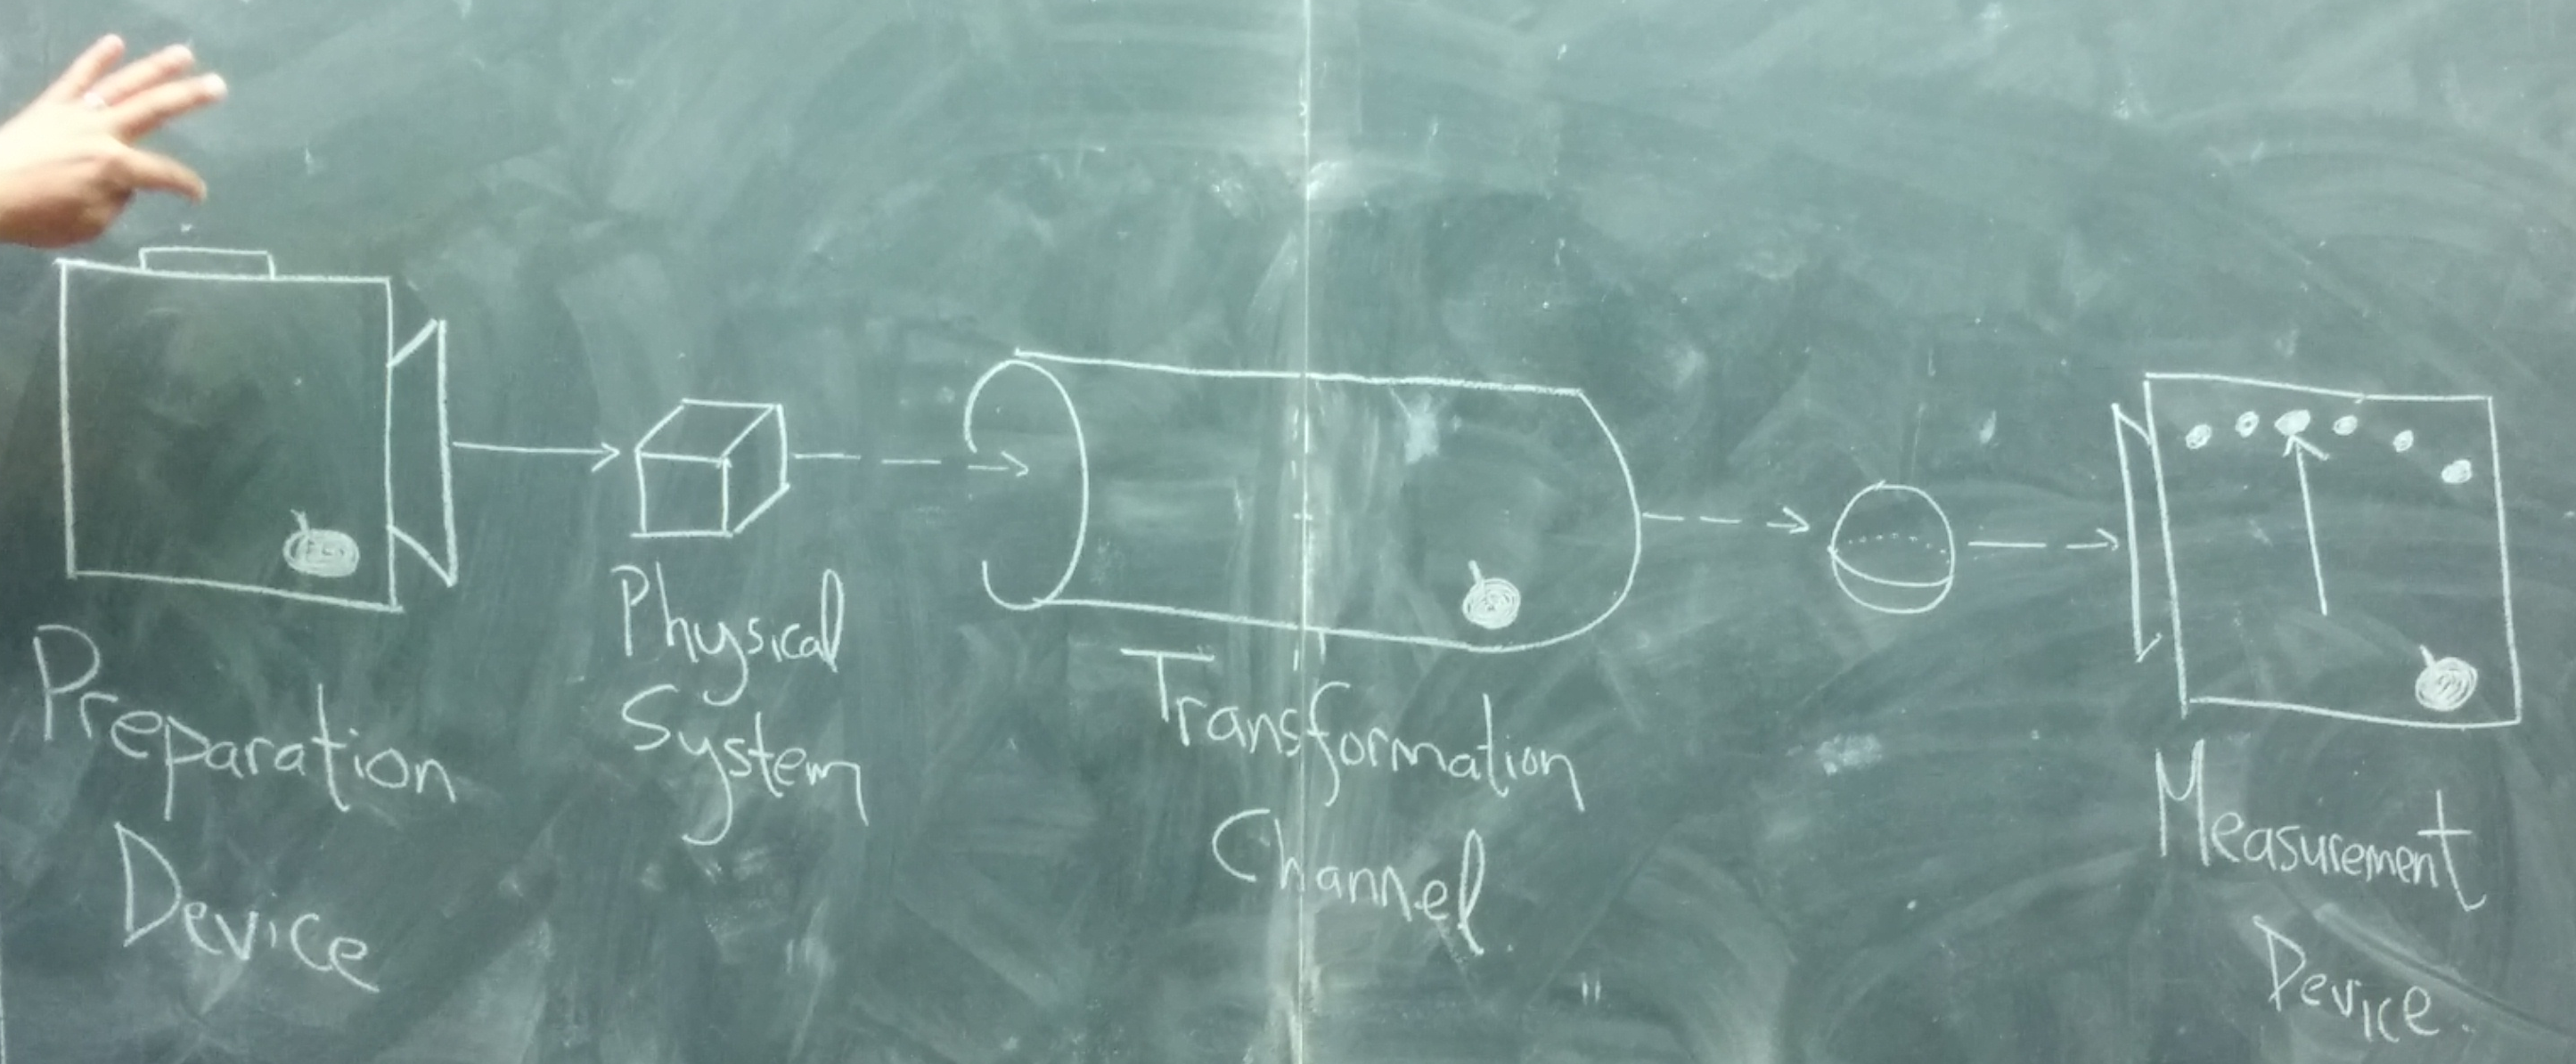
\includegraphics[width=0.8\textwidth]{any_physics.png}
            \caption{"Any physical experiment, classical, quantum, or other, can be viewed as the type of experiment described here." - L. Hardy (2001)}
      \end{figure}

      Axioms for Finite-Dimensional Quantum Mechanics

      \begin{itemize}
        \item Axiom 0. Systems Exist
        \item Axiom 1. For each preparation device $\mathcal{P}$, there is an associated $\ket{\Psi} \in \C^d : \braket{\Psi}{\Psi} = 1$.
        \item Axiom 2. For each transformation channel $\mathcal{T}$, there is an associated $u \in U(\C^d), \ket{\Psi} \rightarrow u\ket{\Psi}$
        \item Axiom 3. For each measurement device $\mathcal{M}$, there is an associated Hermitian $A$ with eigenvalues $\lambda_r$ and eigenkets $\ket{\xi_r}$ such that for input $\ket{\phi}$,
        \[ pr(\lambda_r) = \left| \braket{\phi}{\xi_r}\right|^2 \]
        This is The Born Rule.
      \end{itemize}

      \begin{note}
        $uu^\intercal = \mathbb{1}$ implies unitary, and $A = A^\intercal$ implies hermitian.
      \end{note}

      \begin{exmp}
        Suppose that we have some preparation device with four possible states $\Psi_1, \Psi_2, \Psi_3, \Psi_4$, then we can describe $\Psi_1$ as
        \[ \ket{\Psi_1} = a\ket{+_z} + be^{i\theta}\ket{-_z} \]
        for $a, b \in \R_+$, and $\theta \in [0, 2\pi]$. Then,
        \[ pr(+_z) = \left|\braket{\Psi}{+_z}\right|^2 = a^2\]
        and remember that $a^2 + b^2 = 1$. Also,
        \begin{align*}
          pr(+_x) & = \left| \braket{\Psi}{+_x} \right|^2 \\
                  & = \left| \left( a \bra{+_z}+be^{-i\theta}\bra{-_z} \right) \left( \f{\ket{+_z} + \ket{-_z}}{\sqrt{2}} \right) \right|^2 \\
                  & = \f{1}{2} \left| a + be^{-i\theta} \right|^2 \\
                  & = \f{1}{2} \left( a^2 + b^2 + ab \left( e^{-i\theta} + e^{i\theta} \right) \right) \\
          pr(+_x) & = \f{1}{2} (1 + 2ab\cos\theta)
        \end{align*}

        Using this framework we can find $a_r$, $b_r$, and $\theta_r$ from experimental results (finding $pr(+_x)$, $pr(+_y)$, $pr(+_z)$ for each $\Psi_r$)
      \end{exmp}

      \begin{exmp}
        Prove that $\left|\braket{\Psi}{\phi}\right|^2 = \left|\braket{\tau}{\phi}\right|^2$ where $\ket{\tau} = e^{i\theta} \ket{\Psi}$, for $\ket{\Psi}, \ket{\phi} \in \C^d$.
        \newline
        \begin{align*}
          \left|\braket{\tau}{\phi}\right|^2 & = |e^{-i\theta}|^2\left|\braket{\Psi}{\phi}\right|^2 \\
          & = \left|\braket{\Psi}{\phi}\right|^2 \\ \braket{\tau}{\phi} & = \braket{\Psi}{\phi}
        \end{align*}
      \end{exmp}

     \subsection{Tutorial 5}

       Rememeber the axioms.

        \begin{itemize}
        \item Axiom 0. Systems Exist
        \item Axiom 1. For each preparation device $\mathcal{P}$, there is an associated $\ket{\Psi} \in \C^d : \braket{\Psi}{\Psi} = 1$.
        \item Axiom 2. For each transformation channel $\mathcal{T}$, there is an associated $u \in U(\C^d), \ket{\Psi} \rightarrow u\ket{\Psi}$
        \item Axiom 3. For each measurement device $\mathcal{M}$, there is an associated Hermitian $A = A^\dagger$
      \end{itemize}

      \begin{thrm}
        Let $A \in \mathcal{M}_d(\C): AA^\dagger = A^\dagger A$, then $\exists \lambda_1, \ldots, \lambda_m \in \C, m \leq d$. Then,
        \[ \pi_1,\ldots,\pi_m \in \mathcal{M}_d(\C) : \forall r \in \{1,\ldots,m\}, \pi_r^2 = \pi_r \land \forall r \pm s \pi_r\pi_s = 0. \]
        So,
        \[ A = \sum_{r=1}^m \lambda_r\pi_r \]
        where $\lambda_r$ is a unique eigenvalue of $A$ and $\pi_r$ is an eigenprojector where
        \[ \pi_r = \sum_{s=1}^{\mbox{mult}(\lambda_r)} \ket{\xi_{r_s}{\bra{\xi_{r_s}}}} \]
        for eigenvectors associated with $\lambda_r$.
      \end{thrm}

      So a slight generalization to Axiom 3 is \newline

      \textbf{Axiom 3.} For each $\mathcal{M}$, there is an associated $A = A^\dagger$ such that
      \[ pr(\lambda_r) = \sum_{s=1}^{\mbox{mult}(\lambda_r)} \left| \braket{\Psi}{\xi_{r_s}} \right|^2 \]
      For input $\ket{\Psi}, \ket{\Psi} \longrightarrow \f{\pi_r\ket{\Psi}}{\bra{\Psi}\pi_r\ket{\Psi}}$
      when outcome $\lambda_r$ is registered.

      There we go. My question is, is this just a special case of the unitary axiom?

      \[ \braket{u\Psi}{u\phi} = \bra{\Psi}u^\dagger u\ket{\phi} = \braket{\Psi}{\phi} \]

      Let $\ket{\Psi_1} = \ket{+_z}$ and $\ket{\Psi_2} = \ket{-_z}$ and $\braket{\Psi_1}{\Psi_2} = 0$ and then
      \[ A = \mtx{0 & 1 \\ 1 & 0} \mbox{ \ \ \ \ \ \ $x$ measurement} \]
      Suppose a $+_x$ outcome, then

      \[ \ket{\Psi_1} \rightarrow \ket{+_x}, \ \ \ \ \ket{\Psi_2} \rightarrow \ket{+_x} \ \ \ \braket{+_x}{+_x} = 1 \]

      Let's do an example. Consider the situation in the figure at the bottom:

      Find the values mentioned on the board at the different parts of the experiment. I'm not going to do it but essentially all you need to do is apply the function in the transformation to the input state to get the first one, then given the $+$ outcome occurs the new state just tacks off the $-$ component and is then normalized. Next, do the transformation again and normalize and getting the probability after that is just the same old way of getting probabilities from states. For more of a challenge instead of just measuring twice, say we are measuring $n$ times. This leads to the Quantum Zeno effect becuase we'll notice that as we keep observing the state of system over the course the experiment, we nullify the experiment.

      \begin{figure}[b!]
            \centering
            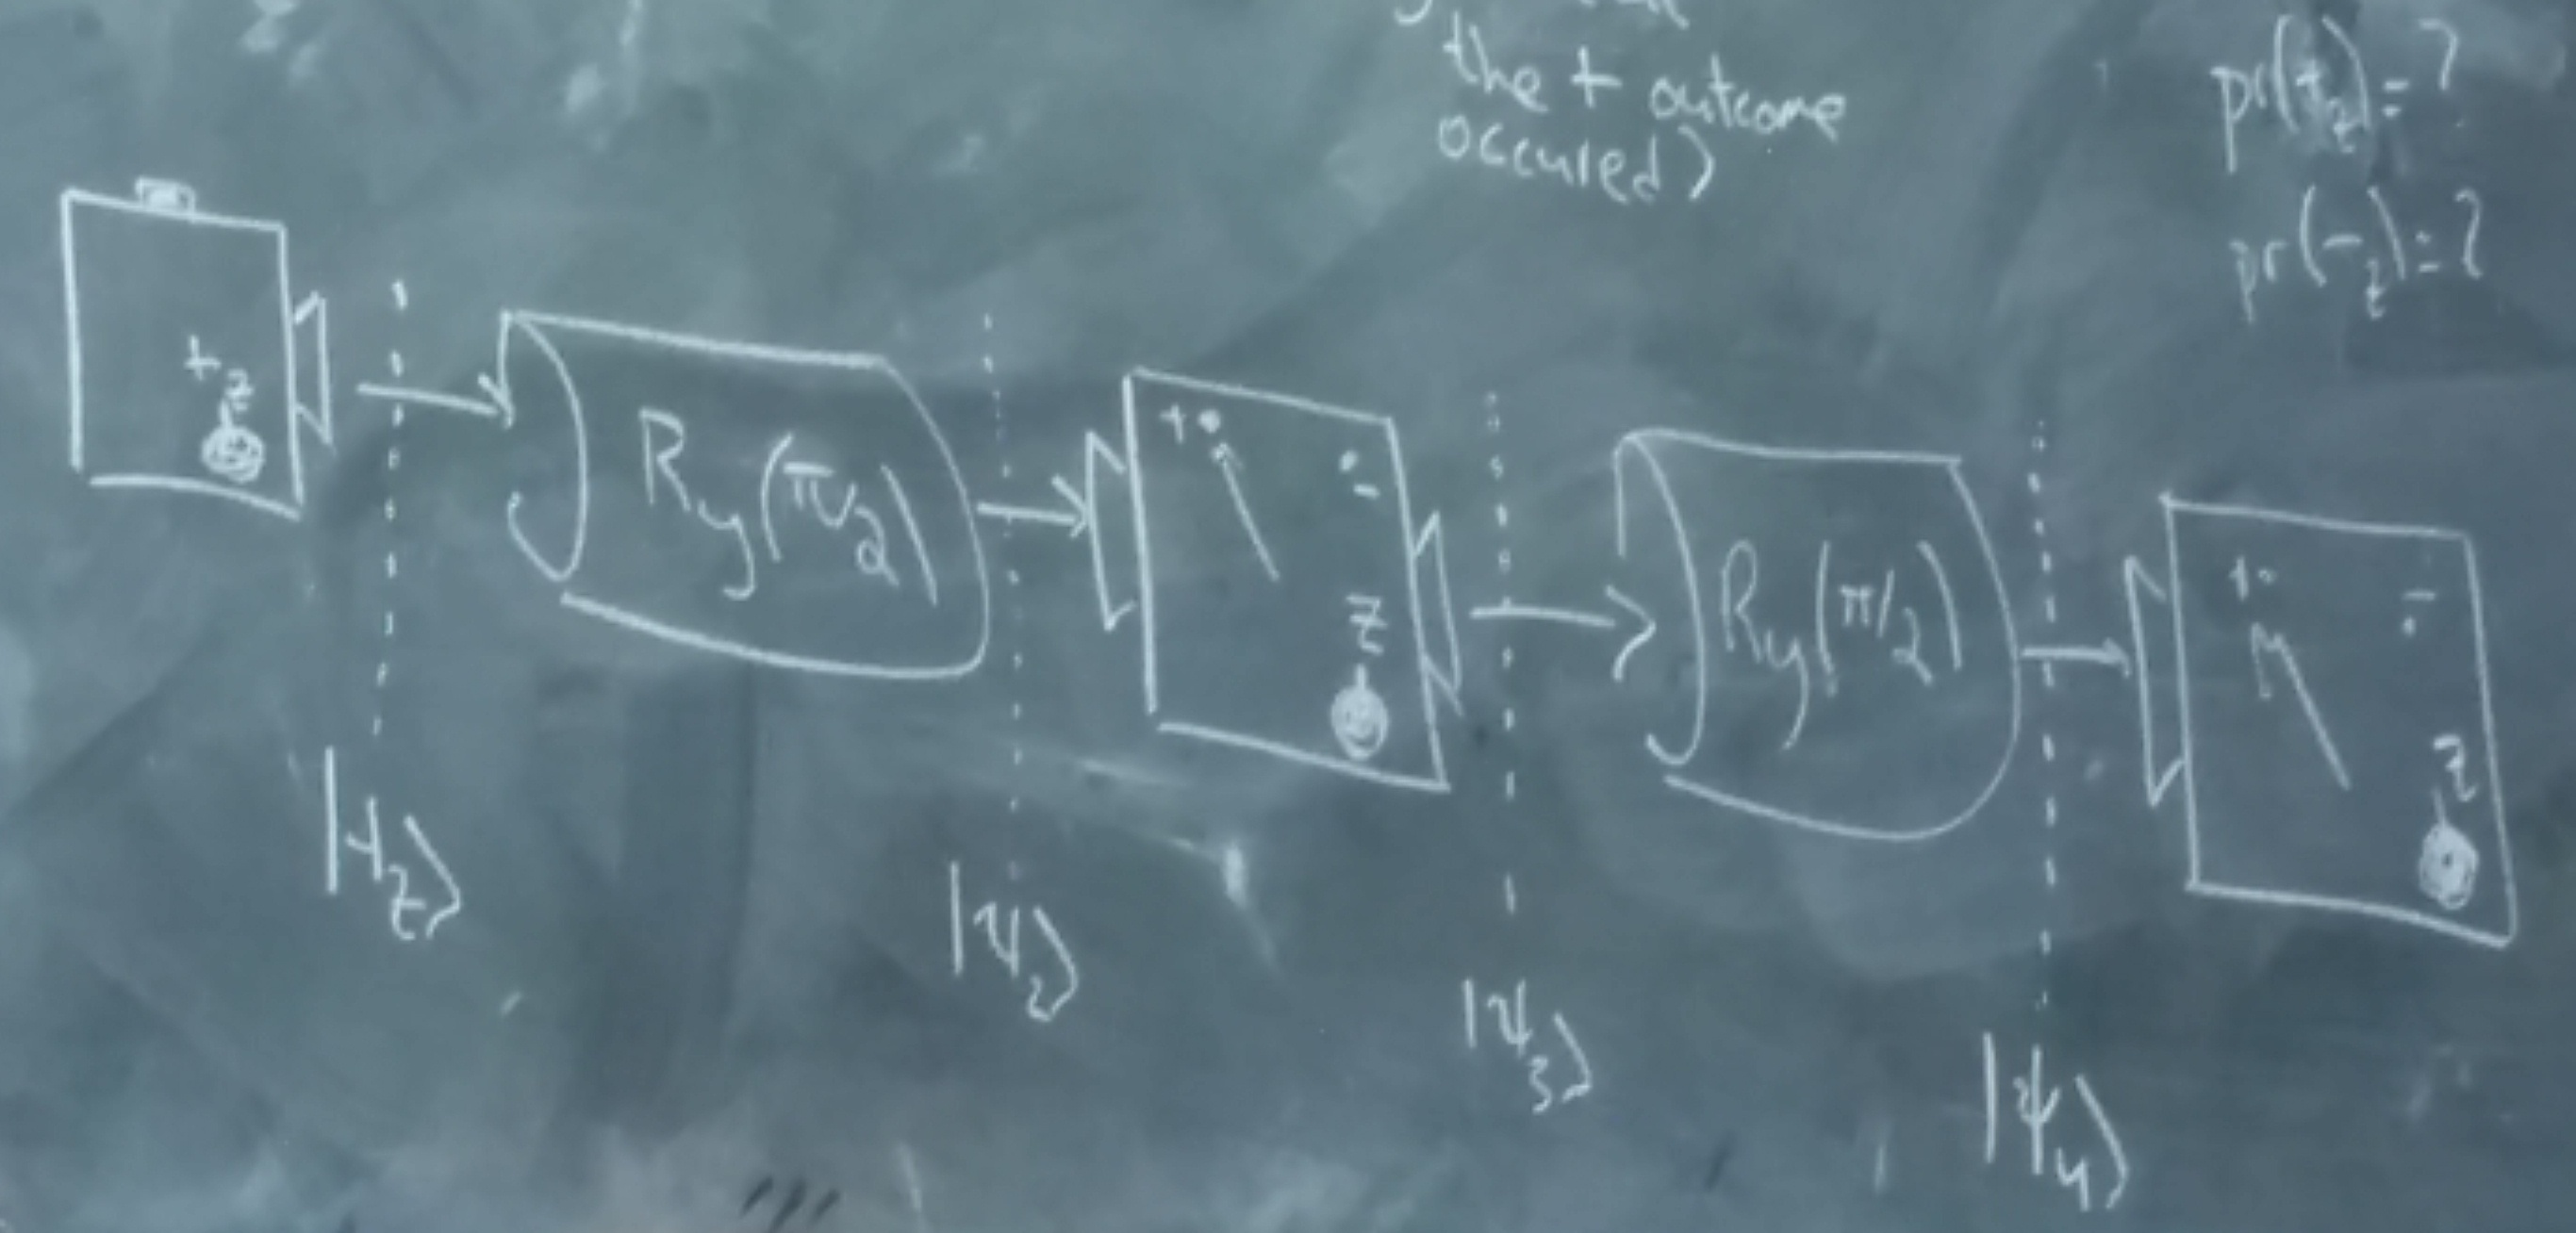
\includegraphics[width=0.8\textwidth]{axiom3_exmp.jpg}
            \caption{Example}
      \end{figure}

  \end{document}
